\documentclass[a4paper, 10pt, fleqn]{article}
%twoside
\usepackage[utf8]{inputenc}
\usepackage[T1]{fontenc}
\usepackage{textcomp}
\usepackage{lmodern}
\usepackage[ngerman]{babel}
\usepackage[nottoc]{tocbibind}
\usepackage{enumerate}
\usepackage{xcolor}
\usepackage{pdfpages}
\usepackage{amsmath}
\usepackage{graphicx}
\usepackage{geometry}
\usepackage{lastpage}
\usepackage[hyphens]{url}
\usepackage{hyperref}
\usepackage{listings}
\usepackage{float}
\usepackage{amssymb}
\usepackage{placeins}
\usepackage{color,soul}
\usepackage{verbatim}
\usepackage{pdflscape}
\usepackage{wrapfig}
\usepackage{paralist}
\usepackage{multicol}
\usepackage{tabu}
\usepackage{tocloft}
\usepackage{soul}
\usepackage[most]{tcolorbox}
\usepackage{ulem}
\usepackage{fancyhdr}
\usepackage{inconsolata}

%Tabelle
\usepackage{booktabs}% nicer horizontal lines$
\usepackage{longtable}
\usepackage{tabularx,colortbl}

%Twoside spacing fix
%\raggedbottom

\renewcommand*{\lstlistoflistings}{%
  \begingroup
  \tocchapter
  \tocfile{\lstlistlistingname}{lol}
  \endgroup
}

\renewcommand*{\listoffigures}{%
  \begingroup
  \tocchapter
  \tocfile{\listfigurename}{lof}
  \endgroup
}

\restylefloat{figure}

\newcommand{\code}[1]{\texttt{#1}}

\renewcommand*{\listoffigures}{%
  \begingroup
  \tocchapter
  \thispagestyle{fancy}
  \tocfile{\listfigurename}{lof}
  \endgroup
}

\geometry{left=3cm, top=3cm, bottom=3cm, right=2cm}

\hypersetup{
    colorlinks,
    linkcolor=black,
    citecolor=black,
    urlcolor=black
}
\tocloftpagestyle{fancy}

\pagestyle{fancy}
\fancyhf{}
\rhead{Diego Bienz}
\lhead{TSM - ProgAlg}
\rfoot{Seite \thepage\ von \pageref{LastPage}}

\definecolor{bluekeywords}{rgb}{0.13,0.13,1}
\definecolor{greencomments}{rgb}{0,0.5,0}
\definecolor{redstrings}{rgb}{0.9,0,0}

\lstset{language=Haskell,
  mathescape=true,
  frame=single,
  numbers=left,                    
  numbersep=5pt,
  numberstyle=\tiny\color{gray},
  rulecolor=\color{black},
  showspaces=false,
  showtabs=false,
  breaklines=true,
  showstringspaces=false,
  breakatwhitespace=true,
  escapeinside={(*@}{@*)},
  tabsize=1,
  commentstyle=\color{greencomments},
  keywordstyle=\color{bluekeywords},
  stringstyle=\color{redstrings},
  basicstyle=\linespread{1}\ttfamily\footnotesize
}

\lstdefinelanguage{OpenCL}
{
morekeywords={__kernel,kernel,__local,local,__global,global,
__constant,constant,__private,private,
char2,char3,char4,char8,char16,
uchar2,uchar3,uchar4,uchar8,uchar16, 
short2,short3,short4,short8,short16, 
ushort2,ushort3,ushort4,ushort8,ushort16, 
int2,int3,int4,int8,int16,
uint2,uint3,uint4,uint8,uint16, 
long2,long3,long4,long8,long16, 
ulong2,ulong3,ulong4,ulong8,ulong16, 
float2,float3,float4,float8,float16, 
image2d_t,image3d_t,sampler_t,event_t, 
bool2,bool3,bool4,bool8,bool16,
half2,half3,half4,half8,half16, 
quad,quad2,quad3,quad4,quad8,quad16, 
complex,imaginary},
  morecomment=[l]{//}, % l is for line comment
  morecomment=[s]{/*}{*/}, % s is for start and end delimiter
  morestring=[b]" % defines that strings are enclosed in double quote
}

\lstdefinelanguage{swift}
{
 language=C++,
  morekeywords={
    func,if,then,else,for,in,while,do,switch,case,default,where,break,continue,fallthrough,return,
    typealias,struct,class,enum,protocol,var,func,let,get,set,willSet,didSet,inout,init,deinit,extension,
    subscript,prefix,operator,infix,postfix,precedence,associativity,left,right,none,convenience,dynamic,
    final,lazy,mutating,nonmutating,optional,override,required,static,unowned,safe,weak,internal,
    private,public,is,as,self,unsafe,dynamicType,true,false,nil,Type,Protocol,
  },
  morecomment=[l]{//}, % l is for line comment
  morecomment=[s]{/*}{*/}, % s is for start and end delimiter
  morestring=[b]" % defines that strings are enclosed in double quotes
}

% Einrücken zu Beginn von neuem Absatz unterdrücken
\setlength{\parindent}{0pt}

% Zeilenabstand einstellen
\usepackage{setspace}
\makeatletter
\newcommand{\MSonehalfspacing}{%
  \setstretch{1.44}%  default
  \ifcase \@ptsize \relax % 10pt
    \setstretch {1.448}%
  \or % 11pt
    \setstretch {1.399}%
  \or % 12pt
    \setstretch {1.433}%
  \fi
}
\newcommand{\MSdoublespacing}{%
  \setstretch {1.92}%  default
  \ifcase \@ptsize \relax % 10pt
    \setstretch {1.936}%
  \or % 11ptEB
    \setstretch {1.866}%
  \or % 12pt
    \setstretch {1.902}%
  \fi
}
\makeatother
\MSonehalfspacing

\newcommand\tightlist


\begin{document}
\begin{titlepage}
%TODO Hier kann die Titelseite erstellt werden

\begin{center}
%\centering
\vspace{1.5cm}
{\scshape\LARGE Hochschule Luzern, T\&A \par}
{\scshape\Large Modul Dokumentation\par}
\vspace{2.0cm}
\title{TSM\_AdvPrPa Fold}
{\huge\bfseries TSM\_AdvPrPa Fold\par}

\vspace{16.0cm}

\end{center}

Autor \\
\textbf{Diego Bienz} \\



\end{titlepage}
\clearpage
\setcounter{tocdepth}{2}
\tableofcontents
\clearpage

% **** Kapitel ab hier
\hypertarget{functional-programming-1}{%
\section{Functional Programming 1}\label{functional-programming-1}}

\hypertarget{correctness}{%
\subsection{Correctness}\label{correctness}}

A program should be correct with respect to its specification. e.g.~a
program that computes the sine perfectly well but should compute the
root is clearly not correct.

One can know wether the program is correct

\begin{itemize}
\tightlist
\item
  by testing

  \begin{itemize}
  \tightlist
  \item
    choose particular input•determine correct result for that input
    using test oracle
  \item
    run program under test on the chosen input
  \item
    compare obtained and correct result
  \end{itemize}
\item
  by proving

  \begin{itemize}
  \tightlist
  \item
    no particular input
  \item
    no execution of the program
  \item
    instead apply mathematical rules to program and specification
  \item
    with a finite number of steps prove that something works for a
    infinite number of values
  \end{itemize}
\end{itemize}

\hypertarget{referential-transparency}{%
\subsection{Referential Transparency}\label{referential-transparency}}

\hypertarget{formal-proof}{%
\subsubsection{Formal proof}\label{formal-proof}}

\begin{figure}[H]
\centering
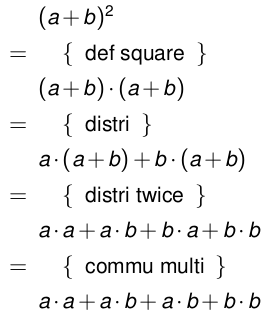
\includegraphics[width=0.25\textwidth]{figures/formalproof1.png}
\caption{Formal proof 1}
\end{figure}

\begin{figure}[H]
\centering
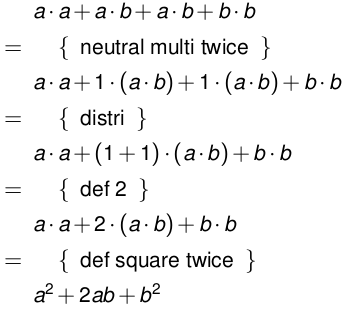
\includegraphics[width=0.25\textwidth]{figures/formalproof2.png}
\caption{Formal proof 2}
\end{figure}

\hypertarget{equality}{%
\subsubsection{Equality}\label{equality}}

\begin{figure}[H]
\centering
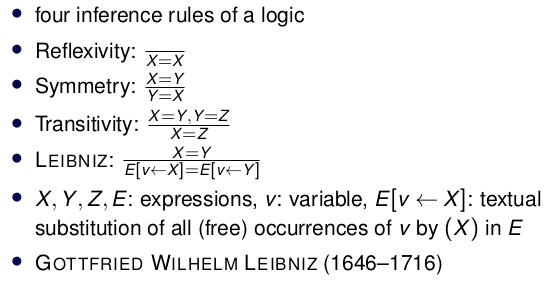
\includegraphics[width=0.5\textwidth]{figures/equality.png}
\caption{Equality}
\end{figure}

\begin{figure}[H]
\centering
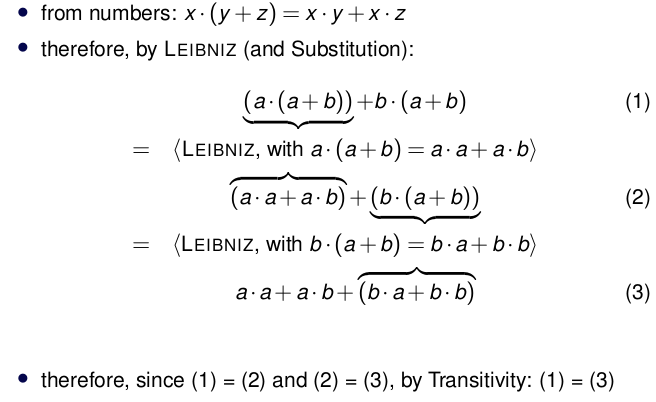
\includegraphics[width=0.5\textwidth]{figures/leibniz.png}
\caption{Example from Leibniz}
\end{figure}

\hypertarget{functional-program}{%
\subsubsection{Functional Program}\label{functional-program}}

\begin{itemize}
\item
  a functional program consists of

  \begin{enumerate}
  \def\labelenumi{\arabic{enumi}.}
  \tightlist
  \item
    a set of value and function declarations
  \item
    a single expression
  \end{enumerate}
\item
  functional programming is referentially transparent

  \begin{itemize}
  \tightlist
  \item
    values and functions are declared via equality
  \item
    equality then means mathematical equality (if using eager evaluation
    modulo termination)
  \end{itemize}
\item
  referential transparency employed for

  \begin{itemize}
  \tightlist
  \item
    program development, transformation, and proof
  \item
    evaluation
  \end{itemize}
\end{itemize}

\clearpage
\hypertarget{imperative-programming}{%
\subsection{Imperative Programming}\label{imperative-programming}}

\begin{itemize}
\tightlist
\item
  syntax: expressions + commands
\item
  semantics: values + environment + state
\item
  expressions are evaluated in the environment and current state,
  yielding a value
\item
  commands are executed in the environment and current state, yielding a
  new state
\item
  Example:

  \begin{itemize}
  \tightlist
  \item
    assignment command with variable v and expression E -\textgreater{}
    v := E
  \item
    E is evaluated in the environment and current state, yielding value
    t; then t is assigned to the storage cell denoted by v in the
    environment, thus yielding a new state
  \end{itemize}
\item
  proofs of imperative programs are well possible too, but are by far
  more complicated
\item
  possible using HOARE logic
\item
  HOARE triple, with P, Q predicates and C command:

  \begin{itemize}
  \tightlist
  \item
    \{P\} C \{Q\}
  \item
    means: if execution of C starts in a state satisfying P, and
    execution terminates, then the resulting state satisfies Q
  \end{itemize}
\item
  Example:

  \begin{itemize}
  \tightlist
  \item
    proof rule for assignment command v := E
  \item
    \{Q{[}v \textless{}- E{]}\} v := E \{Q\}
  \end{itemize}
\end{itemize}

\hypertarget{conclusion-on-imperative-vs.functional}{%
\subsection{Conclusion on Imperative
vs.~Functional}\label{conclusion-on-imperative-vs.functional}}

\textbf{imperative paradigm}

\begin{itemize}
\tightlist
\item
  syntax: expressions + commands
\item
  semantics: values + environment + state
\item
  expressions are evaluated in the environment and current state,
  yielding a value
\item
  commands are executed in the environment and current state, yielding a
  new state
\end{itemize}

\textbf{functional paradigm}

\begin{itemize}
\tightlist
\item
  syntax: expressions
\item
  semantics: values + environment
\item
  expressions are evaluated in the environment, yielding a value
\end{itemize}

\hypertarget{misuse-of-the-symbol-for-equality}{%
\subsubsection{Misuse of the Symbol for Equality
=}\label{misuse-of-the-symbol-for-equality}}

\begin{itemize}
\tightlist
\item
  assignment like x := x + 1 has not the slightest similarity to
  equality
\item
  it is pronounced ``x becomes (gets, receives) x + 1'' \ldots{}
\item
  \ldots{} but never ever ``x equals (is, is equal to) x + 1''
\item
  a different symbol like := or ← should be used instead
\item
  using the symbol for equality = to denote assignment is a horrendous
  design error of too many programming languages.
\end{itemize}

\hypertarget{evaluation}{%
\subsection{Evaluation}\label{evaluation}}

\begin{itemize}
\tightlist
\item
  strategies

  \begin{itemize}
  \tightlist
  \item
    innermost (call-by-value)
  \item
    outermost (call-by-name)
  \item
    \textbf{lazy (outermost + sharing)}
  \item
    reducible expression, or redex
  \item
    application of a function to its argument expressions
  \end{itemize}
\item
  Example: mult(x,y) = x * y

  \begin{itemize}
  \tightlist
  \item
    mult(1+2, 2+3) has three redexes

    \begin{itemize}
    \tightlist
    \item
      1+2, yielding mult(3,2+3)
    \item
      2+3, yielding mult(1+2,5)
    \item
      mult(1+2,2+3) yielding (1+2)*(2+3)
    \end{itemize}
  \end{itemize}
\end{itemize}

\hypertarget{innermost-evaluation}{%
\subsubsection{Innermost Evaluation}\label{innermost-evaluation}}

innermost redex first; if several, choose leftmost one first

mult (1+2,2+3)\\
= mult (3,2+3)\\
= mult (3,5)\\
= 3*5\\
= 15

\clearpage
\hypertarget{outermost-evaluation}{%
\subsubsection{Outermost Evaluation}\label{outermost-evaluation}}

outermost redex first; if several, choose leftmost one first

mult (1+2,2+3)\\
= (1+2) * (2+3)\\
= 3 * (2+3)\\
= 3 * 5\\
= 15

\hypertarget{lazy-evaluation}{%
\subsubsection{Lazy Evaluation}\label{lazy-evaluation}}

Argument expressions might be evaluated more than once if the
corresponding formal parameters occur several times in the body of the
function. Solution to this problem via sharing:

\begin{itemize}
\tightlist
\item
  keep only a single copy of the argument expression, and maintain a
  pointer to it for each corresponding formal parameter
\item
  evaluate the expression once, and replace it by its value
\item
  access this value through the pointers
\end{itemize}

\hypertarget{summary-of-evaluation}{%
\subsubsection{Summary of evaluation}\label{summary-of-evaluation}}

\begin{itemize}
\tightlist
\item
  an argument is evaluated

  \begin{itemize}
  \tightlist
  \item
    innermost: exactly once
  \item
    outermost: zero or more times
  \item
    lazy: at most once
  \end{itemize}
\item
  whenever there exists an order of evaluation that terminates,
  outermost (and thus lazy) evaluation will find it
\end{itemize}

\begin{tcolorbox}[colback=red!5!white,colframe=red!75!black]
The evaluation strategy in which function arguments are evaluated before the function call is made is known as an "eager" evaluation.

Let us postpone evaluating function arguments until after the function call, and then evaluate the argument only if it actually is needed (e.g. if it appears in an expression in the called function). Such a strategy is "lazy."
\end{tcolorbox}

\clearpage
\hypertarget{haskell}{%
\section{Haskell - Introduction}\label{haskell}}

\begin{itemize}
\tightlist
\item
  Functional programming is style of programming in which the basic
  method of computation is the application of functions to arguments;
\item
  A functional language is one that supports and encourages the
  functional style.
\end{itemize}

e.g.~in a computational language like java, summing integers is like:

\begin{lstlisting}[language=Haskell]
int total = 0;
for (int i = 1; i <= 10; i++)
total = total + i;
\end{lstlisting}

in Haskell, it is

\begin{lstlisting}[language=Haskell]
sum [1..10]
\end{lstlisting}

\hypertarget{first-steps}{%
\subsection{First Steps}\label{first-steps}}

Haskell has a compiler and an interpreter as well

\hypertarget{function-application}{%
\subsubsection{Function Application}\label{function-application}}

\begin{lstlisting}[language=Haskell]
f a b + c*d
--Apply the function f to a and b, and add the result to the product of c and d.
\end{lstlisting}

Moreover, function application is assumed to have higher priority than
all other operators.

\begin{figure}[H]
\centering
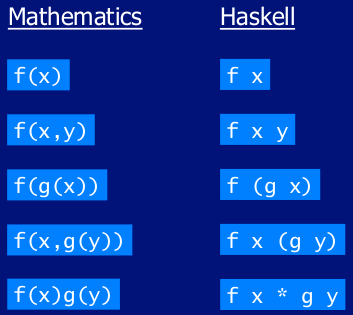
\includegraphics[width=0.3\textwidth]{figures/haskellMath.png}
\caption{Examples}
\end{figure}

\hypertarget{haskell-scripts}{%
\subsubsection{Haskell Scripts}\label{haskell-scripts}}

\begin{itemize}
\tightlist
\item
  New functions are defined within a script, a text file comprising a
  sequence of definitions
\item
  By convention, Haskell scripts usually have a .hs suffix on their
  filename. This is not mandatory, but is useful for identification
  purposes
\item
  To start a script, type in ghci test.hs (test.hs is the script name)
\item
  To use commands within the script, one can type `command-name`
\end{itemize}

\begin{lstlisting}[language=Haskell]
average ns = sum ns `div` length ns
\end{lstlisting}

\clearpage
\hypertarget{haskell}{%
\section{Haskell - Types}\label{haskell}}

Haskell has some basic types, including:

\begin{itemize}
\tightlist
\item
  Bool
\item
  Char
\item
  String
\item
  Int (fixed-precision integers)
\item
  Integer (arbitrary-precision integers)
\item
  Float
\end{itemize}

A list is sequence of values of the same type.

\hypertarget{tuple-types}{%
\subsubsection{Tuple Types}\label{tuple-types}}

A tuple is a sequence of values of different types.

\begin{lstlisting}[language=Haskell]
(False,'a',True) :: (Bool,Char,Bool)
ghci> fst (8,11)  
8  
ghci> snd (8,11)
11
\end{lstlisting}

In difference to the normal type of an array is the type of a tuple
encoding its size.

\hypertarget{function-types}{%
\subsection{Function Types}\label{function-types}}

A function is a mapping from values of one type to values of another type. Functions also have types. When writing our own functions, we can choose to give them an explicit type declaration. This is generally considered to be good practice except when writing very short functions.

\begin{lstlisting}[language=Haskell]
-- "::" is read as "has type of"
not :: Bool -> Bool

removeNonUppercase :: [Char] -> [Char]  
removeNonUppercase st = [ c | c <- st, c `elem` ['A'..'Z']]  
-- meaning that it maps from a string to a string. That's because it takes one string as a parameter and returns another as a result

addThree :: Int -> Int -> Int -> Int  
addThree x y z = x + y + z 
-- The parameters are separated with -> and there's no special distinction between the parameters and the return type.
\end{lstlisting}

\clearpage

\hypertarget{polymorphic-functions}{%
\subsubsection{Polymorphic Functions}\label{polymorphic-functions}}

A function is called polymorphic (``of many forms'') if its type
contains one or more type variables.

\begin{lstlisting}[language=Haskell]
For any type a, length takes a list of values of type a and returns an integer.
\end{lstlisting}

\hypertarget{overloaded-functions}{%
\subsubsection{Overloaded Functions}\label{overloaded-functions}}

A polymorphic function is called overloaded if its type contains one or
more class constraints.

\begin{tcolorbox}[colback=red!5!white,colframe=red!75!black]
For any numeric type a, (+) takes two values of type a and returns a value of type a.
\end{tcolorbox}

\subsection{Type variables}

\begin{lstlisting}[language=Haskell]
ghci> :t head  
head :: [a] -> a

ghci> :t fst  
fst :: (a, b) -> a  
\end{lstlisting}

Types are written in capital case, so it can't exactly be a type. Because it's not in capital case it's actually a type variable. That means that a can be of any type. This is much like generics in other languages, only in Haskell it's much more powerful because it allows us to easily write very general functions if they don't use any specific behavior of the types in them. Functions that have type variables are called polymorphic functions. The type declaration of head states that it takes a list of any type and returns one element of that type.

\clearpage
\subsection{Typeclasses}

If a type is a part of a typeclass, that means that it supports and implements the behavior the typeclass describes.

\begin{lstlisting}[language=Haskell]
ghci> :t (==)  
(==) :: (Eq a) => a -> a -> Bool  
\end{lstlisting}

We see a new thing here, the => symbol. Everything before the => symbol is called a class constraint. We can read the previous type declaration like this: the equality function takes any two values that are of the same type and returns a Bool. The type of those two values must be a member of the Eq class.

\begin{lstlisting}[language=Haskell]
ghci> :t (>)  
(>) :: (Ord a) => a -> a -> Bool 
\end{lstlisting}

Ord is for types that have an ordering. 

\subsection{Operation on Lists}
\label{sec:Operationonlists}
\begin{figure}[H]
\centering
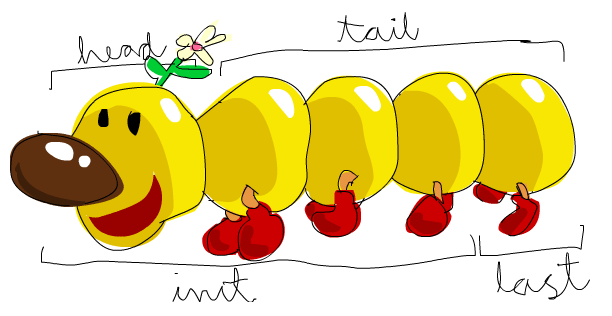
\includegraphics[width=0.5\textwidth]{figures/listOperations.png}
\caption{List operations}
\end{figure}

\begin{lstlisting}[language=Haskell]
ghci> [3,2,1] > [2,1,0]  
True  
ghci> [3,4,2] > [3,4]  
True
ghci> length [5,4,3,2,1]  
5
ghci> null [1,2,3]  
False 
ghci> reverse [5,4,3,2,1]  
[1,2,3,4,5] 
ghci> take 3 [5,4,3,2,1]  
[5,4,3]
ghci> drop 3 [8,4,2,1,5,6]  
[1,5,6] 
ghci> maximum [1,9,2,3,4]  
9  
ghci> sum [5,2,1,6,3,2,5,7]  
31
ghci> 4 `elem` [3,4,5,6]  
True 
ghci> ['a'..'z']  
"abcdefghijklmnopqrstuvwxyz"
ghci> [3,6..20]  
[3,6,9,12,15,18]
take 10 (cycle [1,2,3])  
[1,2,3,1,2,3,1,2,3,1]  
take 10 (repeat 5)  
[5,5,5,5,5,5,5,5,5,5]  
\end{lstlisting}

\clearpage
\hypertarget{haskell}{%
\section{Haskell - Defining Functions}\label{haskell}}

\hypertarget{conditional-expressions}{%
\subsection{Conditional Expressions}\label{conditional-expressions}}

As in most programming languages, functions can be defined using
conditional expressions.

\begin{lstlisting}[language=Haskell]
abs :: Int -> Int
abs n = if n >= 0 then n else -n
\end{lstlisting}

abs takes an integer n and returns n if it is non-negative and -n
otherwise.

Conditional expressions can also be nested:

\begin{lstlisting}[language=Haskell]
signum :: Int -> Int
signum n = if n < 0 then -1 else
if n == 0 then 0 else 1
\end{lstlisting}

\begin{tcolorbox}[colback=red!5!white,colframe=red!75!black]
In Haskell, conditional expressions must always have an else branch.
\end{tcolorbox}

\hypertarget{guarded-equations}{%
\subsubsection{Guarded Equations}\label{guarded-equations}}

As an alternative to conditionals, functions can also be defined using
guarded equations

\begin{lstlisting}[language=Haskell]
abs n | n >= 0 = n
      | otherwise = -n
\end{lstlisting}

Guarded equations can be used to make definitions involving multiple
conditions easier to read.

\hypertarget{pattern-matching}{%
\subsection{Pattern Matching}\label{pattern-matching}}

Many functions have a particularly clear definition using pattern matching on their arguments.

\begin{lstlisting}[language=Haskell]
lucky :: (Integral a) => a -> String  
lucky 7 = "LUCKY NUMBER SEVEN!"  
lucky x = "Sorry, you're out of luck, pal!" 
\end{lstlisting}

When you call lucky, the patterns will be checked from top to bottom and when it conforms to a pattern, the corresponding function body will be used. The only way a number can conform to the first pattern here is if it is 7. If it's not, it falls through to the second pattern, which matches anything and binds it to x.

\begin{lstlisting}[language=Haskell]
factorial :: (Integral a) => a -> a  
factorial 0 = 1  
factorial n = n * factorial (n - 1) 

addVectors :: (Num a) => (a, a) -> (a, a) -> (a, a)  
addVectors a b = (fst a + fst b, snd a + snd b)  
--addVectors (x1, y1) (x2, y2) = (x1 + x2, y1 + y2)
\end{lstlisting}

\begin{tcolorbox}[colback=red!5!white,colframe=red!75!black]
The underscore symbol \_ is a wildcard pattern that matches any argument value.
Patterns are matched in order.
Patterns may not repeat variables
\end{tcolorbox}

\hypertarget{list-patterns}{%
\subsubsection{List Patterns}\label{list-patterns}}

Since [1,2,3] is just syntactic sugar for 1:2:3:[], you can also use the former pattern. A pattern like x:xs will bind the head of the list to x and the rest of it to xs, even if there's only one element so xs ends up being an empty list. 

\begin{tcolorbox}[colback=red!5!white,colframe=red!75!black]
[1,2,3,4] means internal actually 1:(2:(3:(4:[]))). <- Syntactic Sugar
\end{tcolorbox}

Functions on lists can be defined using x:xs patterns. For more operations on lists refer to chapter \ref{sec:Operationonlists}.

\begin{lstlisting}[language=Haskell]
head :: [a] -> a
head (x:_) = x
tail :: [a] -> [a]
tail (_:xs) = xs

head' :: [a] -> a  
head' [] = error "Can't call head on an empty list, dummy!"  
head' (x:_) = x  

ghci> let xs = [(1,3), (4,3), (2,4), (5,3), (5,6), (3,1)]  
ghci> [a+b | (a,b) <- xs]  
[4,7,6,8,11,4]  
\end{lstlisting}

\subsection{Guard}

Whereas patterns are a way of making sure a value conforms to some form and deconstructing it, guards are a way of testing whether some property of a value (or several of them) are true or false. Guards are indicated by pipes that follow a function's name and its parameters. A guard is basically a boolean expression. If it evaluates to True, then the corresponding function body is used. If it evaluates to False, checking drops through to the next guard and so on. Many times, the last guard is otherwise. otherwise is defined simply as otherwise = True and catches everything. 

Guards can also be written inline, although I'd advise against that because it's less readable, even for very short functions.

\begin{lstlisting}[language=Haskell]
bmiTell :: (RealFloat a) => a -> a -> String  
bmiTell weight height  
    | bmi <= skinny = "You're underweight, you emo, you!"  
    | bmi <= 25.0 = "You're supposedly normal. Pffft, I bet you're ugly!"  
    | bmi <= 30.0 = "You're fat! Lose some weight, fatty!"  
    | otherwise   = "You're a whale, congratulations!"  
    where bmi = weight / height ^ 2 
          skinny = 18.5  

max' :: (Ord a) => a -> a -> a  
max' a b | a > b = a | otherwise = b  
\end{lstlisting}

We put the keyword \textbf{where} after the guards (usually it's best to indent it as much as the pipes are indented) and then we define several names or functions. These names are visible across the guards and give us the advantage of not having to repeat ourselves.

\clearpage
\subsection{Let Statement}

The form is let <bindings> in <expression>. The names that you define in the let part are accessible to the expression after the \textbf{in} part. Let bindings are expressions and are fairly local in their scope, they can't be used across guards (which \textit{where} can.

\begin{lstlisting}[language=Haskell]
cylinder :: (RealFloat a) => a -> a -> a  
cylinder r h = 
    let sideArea = 2 * pi * r * h  
        topArea = pi * r ^2  
    in  sideArea + 2 * topArea  
    
--Different variables are seperated with semikolon.
ghci> (let a = 100; b = 200; c = 300 in a*b*c, let foo="Hey "; bar = "there!" in foo ++ bar)  
(6000000,"Hey there!") 
\end{lstlisting}

\hypertarget{lambda-expressions}{%
\subsection{Lambda Expressions}\label{lambda-expressions}}

Functions can be constructed without naming the functions by using
lambda expressions.

\begin{lstlisting}[language=Haskell]
$\lambda$x -> x + x
\end{lstlisting}

The symbol $\lambda$ is the Greek letter lambda, and is typed at the keyboard as a backslash \textbackslash{}.

\begin{itemize}
\tightlist
\item
  Lambda expressions can be used to give a formal meaning to functions
  defined using currying
\item
  Lambda expressions are also useful when defining functions that return
  functions as results
\item
  Lambda expressions can be used to avoid naming functions that are only
  referenced once
\end{itemize}

\hypertarget{operator-sections}{%
\subsection{Operator Sections}\label{operator-sections}}

An operator written between its two arguments can be converted into a
curried function written before its two arguments by using parentheses.

\begin{lstlisting}[language=Haskell]
> 1+2
3
> (+) 1 2
3

or
> (1+) 2
3
\end{lstlisting}

In general, if $\oplus$ is an operator then functions of the form ($\oplus$), (x$\oplus$) and (y$\oplus$) are called sections.

\clearpage

\hypertarget{haskell}{%
\section{Haskell - List Comprehensions}\label{haskell}}

In Haskell, a comprehension notation can be used to construct new lists
from old lists.

\begin{lstlisting}[language=Haskell]
ghci> [x*2 | x <- [1..10], x*2 >= 12]  
[12,14,16,18,20]

boomBangs xs = [ if x < 10 then "BOOM!" else "BANG!" | x <- xs, odd x]
ghci> boomBangs [5..15]
["BOOM!","BOOM!","BOOM!","BANG!","BANG!","BANG!"]

[(x,y) | y <- [4,5], x <- [1,2,3]]
[(1,4),(2,4),(3,4),(1,5),(2,5),(3,5)]

ghci> let nouns = ["hobo","frog","pope"]  
ghci> let adjectives = ["lazy","grouchy","scheming"]  
ghci> [adjective ++ " " ++ noun | adjective <- adjectives, noun <- nouns]  
["lazy hobo","lazy frog","lazy pope","grouchy hobo","grouchy frog","grouchy pope","scheming hobo","scheming frog","scheming pope"]   
\end{lstlisting}

\begin{itemize}
\tightlist
\item
  The expression x ← {[}1..5{]} is called a generator, as it states how
  to generate values for x
\item
  Comprehensions can have multiple generators, separated by commas
\item
  Changing the order of the generators changes the order of the elements
  in the final list
\item
  Multiple generators are like nested loops, with later generators as
  more deeply nested loops whose variables change value more frequently
\end{itemize}

\hypertarget{dependant-generators}{%
\subsubsection{Dependant Generators}\label{dependant-generators}}

Later generators can depend on the variables that are introduced by
earlier generators. Using a dependant generator we can define the
library function that concatenates a list of lists.

\begin{lstlisting}[language=Haskell]
concat :: [[a]] -> [a]
concat xss = [x | xs <- xss, x <- xs]

concat [[1,2,3],[4,5],[6]]
[1,2,3,4,5,6]
\end{lstlisting}

\hypertarget{guards}{%
\subsubsection{Guards (Predicates)}\label{guards}}

List comprehensions can use guards to restrict the values produced by
earlier generators.

\begin{lstlisting}[language=Haskell]
ghci> [x | x <- [1..10], even x]
[2,4,6,8,10]

--Multiple predicates are seperated by comma
ghci> [ x | x <- [10..20], x /= 13, x /= 15, x /= 19]  
[10,11,12,14,16,17,18,20] 
\end{lstlisting}

\hypertarget{the-zip-function}{%
\subsection{The Zip Function}\label{the-zip-function}}

A useful library function is zip, which maps two lists to a list of
pairs of their corresponding elements.

\begin{lstlisting}[language=Haskell]
zip :: [a] -> [b] -> [(a,b)]
> zip ['a','b','c'] [1,2,3,4]
[('a',1),('b',2),('c',3)]
\end{lstlisting}

\clearpage
\hypertarget{string-comprehensions}{%
\subsection{String Comprehensions}\label{string-comprehensions}}

\begin{itemize}
\tightlist
\item
  A string is a sequence of characters enclosed in double quotes.
  Internally, however, strings are represented as lists of characters.
\item
  Because strings are just special kinds of lists, any polymorphic
  function that operates on lists can also be applied to strings.
\item
  Similarly, list comprehensions can also be used to define functions on
  strings, such counting how many times a character occurs in a string:
\end{itemize}

\begin{lstlisting}[language=Haskell]
count :: Char -> String -> Int
count x xs = length [x' | x' <- xs, x == x']

--Own version of length
length' xs = sum [1 | _ <- xs]   

removeNonUppercase st = [ c | c <- st, c `elem` ['A'..'Z']] 
ghci> removeNonUppercase "Hahaha! Ahahaha!"  
"HA"
\end{lstlisting}

\clearpage
\hypertarget{haskell}{%
\section{Haskell - Recursive Functions}\label{haskell}}

In Haskell, functions can also be defined in terms of themselves. Such
functions are called recursive.

\begin{itemize}
\tightlist
\item
  Some functions, such as factorial, are simpler to define in terms of
  other functions.
\item
  As we shall see, however, many functions can naturally be defined in
  terms of themselves.
\item
  Properties of functions defined using recursion can be proved using
  the simple but powerful mathematical technique of induction.
\end{itemize}

\hypertarget{recursion-on-lists}{%
\subsection{Recursion on Lists}\label{recursion-on-lists}}

\begin{lstlisting}[language=Haskell]
product :: Num a -> [a] -> a
product [] = 1
product (n:ns) = n * product ns

In execution:

product [2,3,4]
2 * product [3,4]
2 * (3 * product [4])
2 * (3 * (4 * product []))
2 * (3 * (4 * 1))
24

--or
-- The maximum function takes a list of things that can be ordered (e.g. instances of the Ord typeclass) and returns the biggest of them.

maximum' :: (Ord a) => [a] -> a  
maximum' [] = error "maximum of empty list"  
maximum' [x] = x  
maximum' (x:xs)   
    | x > maxTail = x  
    | otherwise = maxTail  
    where maxTail = maximum' xs
\end{lstlisting}

\hypertarget{multiple-arguments}{%
\subsection{Multiple Arguments}\label{multiple-arguments}}

Functions with more than one argument can also be defined using
recursion.

\begin{lstlisting}[language=Haskell]
zip :: [a] -> [b] -> [(a,b)]
zip []    _       = []
zip  _    []      = []
zip (x:xs) (y:ys) = (x,y) : zip xs ys
\end{lstlisting}

\subsection{Some Examples}

\begin{lstlisting}[language=Haskell]
take' :: (Num i, Ord i) => i -> [a] -> [a]  
take' n _  
    | n <= 0   = []  
take' _ []     = []  
take' n (x:xs) = x : take' (n-1) xs 

reverse' :: [a] -> [a]  
reverse' [] = []  
reverse' (x:xs) = reverse' xs ++ [x]
\end{lstlisting}

\clearpage
\subsection{Quick Sort}

We have a list of items that can be sorted. Their type is an instance of the \textbf{Ord} typeclass. The edge condition is the empty list. Now a sorted list is a list that has all the values smaller than (or equal to) the head of the list in front (and those values are sorted), then comes the head of the list in the middle and then come all the values that are bigger than the head (they're also sorted).

\begin{lstlisting}[language=Haskell]
quicksort :: (Ord a) => [a] -> [a]  
quicksort [] = []  
quicksort (x:xs) =   
    let smallerSorted = quicksort [a | a <- xs, a <= x]  
        biggerSorted = quicksort [a | a <- xs, a > x]  
    in  smallerSorted ++ [x] ++ biggerSorted  
\end{lstlisting}

So if we have, say [5,1,9,4,6,7,3] and we want to sort it, this algorithm will first take the head, which is 5 and then put it in the middle of two lists that are smaller and bigger than it. So at one point, you'll have [1,4,3] ++ [5] ++ [9,6,7]. We know that once the list is sorted completely, the number 5 will stay in the fourth place since there are 3 numbers lower than it and 3 numbers higher than it. Now, if we sort [1,4,3] and [9,6,7], we have a sorted list! We sort the two lists using the same function. Eventually, we'll break it up so much that we reach empty lists and an empty list is already sorted in a way, by virtue of being empty.

\clearpage
\hypertarget{haskell}{%
\section{Haskell - Higher-Order Functions}\label{haskell}}

Haskell functions can take functions as parameters and return functions as return values. A function that does either of those is called a higher order function.


\hypertarget{curried-functions}{%
\subsection{Curried Functions}\label{curried-functions}}

Functions with multiple arguments are also possible by returning
functions as results. Functions that take their arguments one at a time
are called \textbf{curried functions}.

\begin{lstlisting}[language=Haskell]
ghci> max 4 5  
5 
max :: (Ord a) => a -> a -> a
-- Can also be written like: max :: (Ord a) => a -> (a -> a)

multThree :: (Num a) => a -> a -> a -> a  
multThree x y z = x * y * z
\end{lstlisting}

Curried functions are more flexible than functions on tuples, because
useful functions can often be made by partially applying a curried
function.

\hypertarget{currying-conventions}{%
\subsubsection{Currying Conventions}\label{currying-conventions}}

\begin{enumerate}
\def\labelenumi{\arabic{enumi}.}
\tightlist
\item
  The arrow -\textgreater{} associates to the right.
\item
  As a consequence, it is then natural for function application to
  associate to the left
\end{enumerate}

\begin{tcolorbox}[colback=red!5!white,colframe=red!75!black]
Unless tupling is explicitly required, all functions in Haskell are normally defined in curried form.
\end{tcolorbox}

\subsubsection{Currying infix functions}

Infix functions can also be partially applied by using sections. To section an infix function, simply surround it with parentheses and only supply a parameter on one side. That creates a function that takes one parameter and then applies it to the side that's missing an operand.

\begin{lstlisting}[language=Haskell]
ghci> max 4 5  
5 
max :: (Ord a) => a -> a -> a
-- Can also be written like: max :: (Ord a) => a -> (a -> a)

multThree :: (Num a) => a -> a -> a -> a  
multThree x y z = x * y * z
\end{lstlisting}

\clearpage
\subsection{Higher-Order function declaration}

\begin{lstlisting}[language=Haskell]
applyTwice :: (a -> a) -> a -> a  
applyTwice f x = f (f x)  
\end{lstlisting}

Before, we didn't need parentheses because -> is naturally right-associative. However, here, they're mandatory. They indicate that the first parameter is a function that takes something and returns that same thing. The second parameter is something of that type also and the return value is also of the same type. We could read this type declaration in the curried way, but to save ourselves a headache, we'll just say that this function takes two parameters and returns one thing. The first parameter is a function (of type a -> a) and the second is that same a.

\begin{lstlisting}[language=Haskell]
zipWith' :: (a -> b -> c) -> [a] -> [b] -> [c]  
zipWith' _ [] _ = []  
zipWith' _ _ [] = []  
zipWith' f (x:xs) (y:ys) = f x y : zipWith' f xs ys  

ghci> zipWith' (+) [4,2,5,6] [2,6,2,3]  
[6,8,7,9]  
\end{lstlisting}

The function zipWith' takes a function and two lists as parameters and then joins the two lists by applying the function between corresponding elements.

\hypertarget{map-function}{%
\subsection{Map Function}\label{map-function}}

The higher-order library function called map applies a function to every
element of a list.

\begin{lstlisting}[language=Haskell]
map :: (a -> b) -> [a] -> [b]

> map (+1) [1,3,5,7]
[2,4,6,8]
\end{lstlisting}

\hypertarget{filter-function}{%
\subsection{Filter Function}\label{filter-function}}

The higher-order library function filter selects every element from a
list that satisfies a predicate.

\begin{lstlisting}[language=Haskell]
filter :: (a -> Bool) -> [a] -> [a]

> filter even [1..10]
[2,4,6,8,10]
\end{lstlisting}

\clearpage
\hypertarget{foldr-function-folg-right}{%
\subsection{Foldr Function (Folg
right)}\label{foldr-function-folg-right}}

\begin{lstlisting}[language=Haskell]
f [] = v  //Neutral Element
f (x:xs) = x $\oplus$ f xs
\end{lstlisting}

f maps the empty list to some value v (Default value), and any non-empty
list to some function $\oplus$  applied to its head and f of its tail.

\begin{lstlisting}[language=Haskell]
//Example
sum = foldr (+) 0
\end{lstlisting}

\begin{figure}[H]
\centering
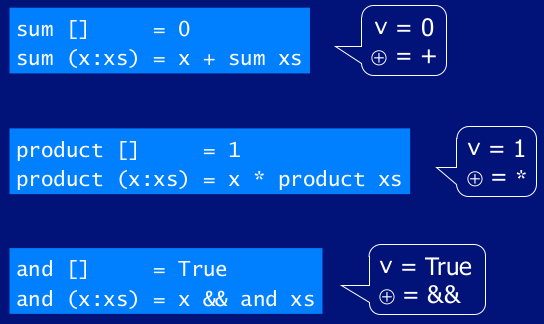
\includegraphics[width=0.5\textwidth]{figures/fold_examples.png}
\caption{Foldr examples}
\end{figure}

\begin{figure}[H]
\centering
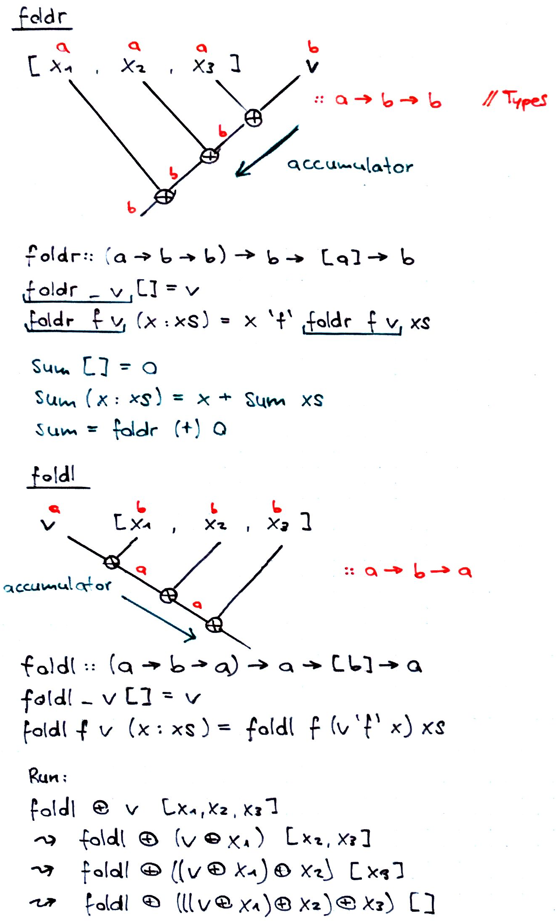
\includegraphics[width=0.7\textwidth]{figures/foldr.png}
\caption{Foldr}
\end{figure}

\hypertarget{other-library-functions}{%
\subsection{Other Library Functions}\label{other-library-functions}}

The library function (.) returns the composition of two functions as a
single function.

\begin{lstlisting}[language=Haskell]
(.) :: (b -> c) -> (a -> b) -> (a -> c)
f . g = $\lambda$x -> f (g x)

example:
odd :: Int -> Bool
odd = not . even
\end{lstlisting}

\hypertarget{all}{%
\subsubsection{all}\label{all}}

The library function all decides if every element of a list satisfies a
given predicate.

\begin{lstlisting}[language=Haskell]
> all even [2,4,6,8,10]
True
\end{lstlisting}

\hypertarget{any}{%
\subsubsection{any}\label{any}}

Dually, the library function any decides if at least one element of a
list satisfies a predicate.

\begin{lstlisting}[language=Haskell]
> any (== ' ') "abc def"
True
\end{lstlisting}

\hypertarget{takewhile}{%
\subsubsection{takeWhile}\label{takewhile}}

The library function takeWhile selects elements from a list while a
predicate holds of all the elements.

\begin{lstlisting}[language=Haskell]
> takeWhile (/= ' ') "abc def"
"abc"
\end{lstlisting}


\clearpage
\hypertarget{haskell}{%
\section{Haskell - Declaring Types and Classes}\label{haskell}}

\hypertarget{type-declarations}{%
\subsection{Type Declarations}\label{type-declarations}}

In Haskell, a new name for an \textbf{existing} type can be defined
using a type declaration. (not new type)

\begin{lstlisting}[language=Haskell]
type String = [Char]
--or
type Pos = (Int,Int)
\end{lstlisting}

Like function definitions, type declarations can also have parameters.
For example, given

\begin{lstlisting}[language=Haskell]
type Pair a = (a,a)
\end{lstlisting}

Type declarations can be nested, but not recursive.

\begin{lstlisting}[language=Haskell]
--Allowed
type Pos = (Int,Int)
type Trans = Pos -> Pos

--Not allowed
type Tree = (Int,[Tree])
\end{lstlisting}

\hypertarget{data-declarations}{%
\subsection{Data Declarations}\label{data-declarations}}

A completely \textbf{new} type can be defined by specifying its values
using a data declaration.

\begin{lstlisting}[language=Haskell]
data Bool = False | True
\end{lstlisting}

\begin{itemize}
\tightlist
\item
  The two values False and True are called the constructors for the type
  Bool.
\item
  Type and constructor names must always begin with an upper-case
  letter.
\item
  Data declarations are similar to context free grammars. The former
  specifies the values of a type, the latter the sentences of a
  language.
\end{itemize}

\hypertarget{constructor}{%
\subsubsection{Constructor}\label{constructor}}

The constructors in a data declaration can also have parameters. For
example, given

\begin{lstlisting}[language=Haskell]
data Shape  = Circle Float
            | Rect Float Float
\end{lstlisting}

we can define

\begin{lstlisting}[language=Haskell]
square :: Float -> Shape
square n = Rect n n
area :: Shape -> Float
area (Circle r) = pi * r^2
area (Rect x y) = x * y
\end{lstlisting}

Not surprisingly, data declarations themselves can also have parameters.
For example, given

\begin{lstlisting}[language=Haskell]
data Maybe a = Nothing | Just a
\end{lstlisting}

we can define

\begin{lstlisting}[language=Haskell]
safediv :: Int -> Int -> Maybe Int
safediv _ 0 = Nothing
safediv m n = Just (m `div` n)
safehead :: [a] -> Maybe a
safehead [] = Nothing
safehead xs = Just (head xs)
\end{lstlisting}

\hypertarget{recursive-types}{%
\subsection{Recursive Types}\label{recursive-types}}

In Haskell, new types can be declared in terms of themselves. That is,
types can be recursive.

\begin{lstlisting}[language=Haskell]
data Nat = Zero | Succ Nat
--Nat is either zero or a successor of Nat
\end{lstlisting}

e.g.~Succ (Succ (Succ Zero)) = 3.

\hypertarget{binary-trees}{%
\subsection{Binary Trees}\label{binary-trees}}

A binary tree is a two-way branching structure. Using recursion, a
suitable new type to represent such binary trees can be declared by:

\begin{lstlisting}[language=Haskell]
data Tree a = Leaf a
            | Node (Tree a) a (Tree a)
\end{lstlisting}

\begin{figure}[H]
\centering
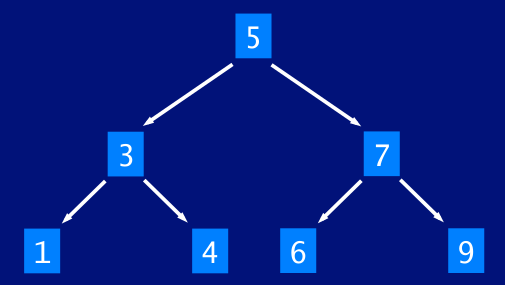
\includegraphics[width=0.5\textwidth]{figures/binaryTreeExample.png}
\caption{Tree Example}
\end{figure}

This tree could be represented with

\begin{lstlisting}[language=Haskell]
t :: Tree Int
t = Node (Node (Leaf 1) 3 (Leaf 4)) 5
(Node (Leaf 6) 7 (Leaf 9))
22
\end{lstlisting}

\clearpage
\hypertarget{haskell}{%
\section{Haskell - Interactive Programming}\label{haskell}}

\hypertarget{io-functions}{%
\subsection{IO functions}\label{io-functions}}

It is possible to interact with the real world from Haskell. You are
able to develop functions which return an IO of a type.

\begin{itemize}
\tightlist
\item
  Normal Haskell functions are pure (without side effects)
\item
  If you want to interact with the outsite world, you have to use IO
\item
  The IO seperates the pure Haskell functions from side effects
\item
  Haskell executes the function and returns the IO of a specific type,
  which then can be used to interact with the outside world.
\end{itemize}

\begin{figure}[H]
\centering
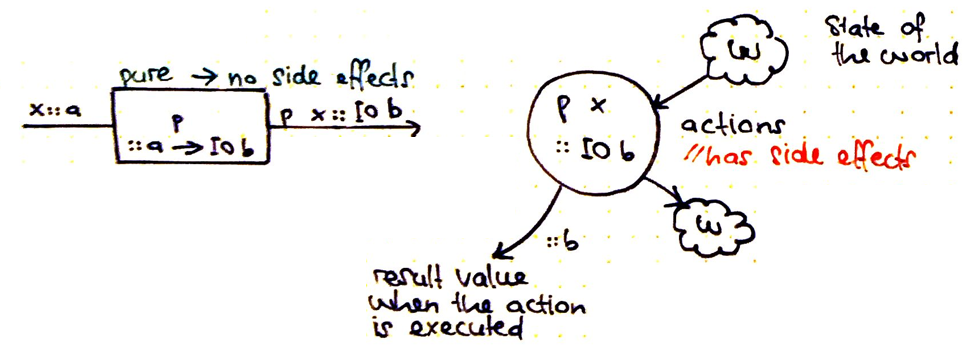
\includegraphics[width=1\textwidth]{figures/pureHaskellFunctions.png}
\caption{Pure Functions}
\end{figure}

\begin{figure}[H]
\centering
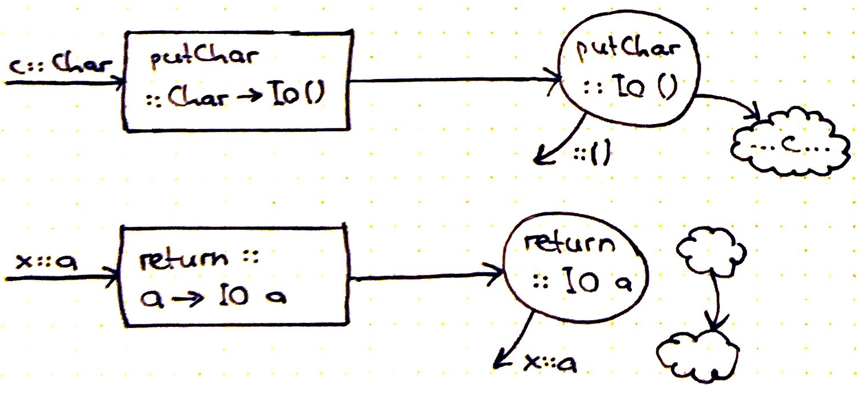
\includegraphics[width=1\textwidth]{figures/ioHaskellFunction.png}
\caption{IO Function}
\end{figure}

\begin{figure}[H]
\centering
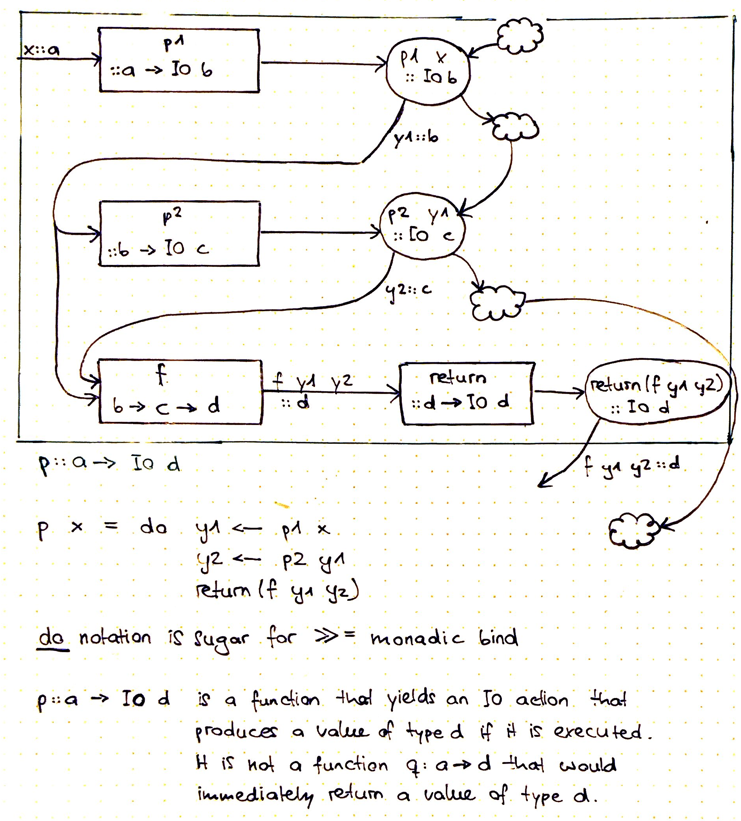
\includegraphics[width=1\textwidth]{figures/doHaskell.png}
\caption{Do Haskell}
\end{figure}

With the do notation, one is able to interact with the world multiple
times and concatonate the actions.

\textbf{p :: a -\textgreater{} IO d} is a function that yields an IO
action that produces a value of type d if the IO is executed. It is not
a function \textbf{q : a -\textgreater{} d} that would immediately
return a value of type d.

\clearpage
\hypertarget{haskell}{%
\section{Haskell - Interpreter}\label{haskell}}

\begin{tcolorbox}[colback=red!5!white,colframe=red!75!black]
TODO: Ich verstehe nicht ganz, was der Interpeter mit Haskell zu tun hat bzw. für was wir das gemacht haben.
\end{tcolorbox}

\hypertarget{abstract-operator}{%
\subsection{Abstract Operator}\label{abstract-operator}}

Instead of using expressions directly, one can replace them with
abstract syntax. For instance instead of using arithmetic operators, one
can define a data type `ArithOperator'.

\begin{lstlisting}[language=Haskell]
type Ident = String

data ArithOperator
= Times
| Div
| Mod
| Plus
| Minus
deriving (Eq, Show)

data ArithExpr
= LitAExpr Int
| IdAExpr Ident
| DyaAExpr ArithOperator ArithExpr ArithExpr

evalAOpr :: ArithOperator -> (Value -> Value -> Value)
evalAOpr Times = (*)
evalAOpr Div = div
evalAOpr Mod = mod
evalAOpr Plus = (+)
evalAOpr Minus = (-)

testExp1 = DyaAExpr Plus (LitAExpr 1) (DyaAExpr Times (LitAExpr 2) (LitAExpr 3))
\end{lstlisting}

\hypertarget{concrete-versus-abstract-syntax}{%
\subsubsection{Concrete Versus Abstract
Syntax}\label{concrete-versus-abstract-syntax}}

\begin{itemize}
\tightlist
\item
  Concrete syntax is easier to read for humans
\item
  Abstract syntax is easier to process for machines
\end{itemize}

\hypertarget{semantic-values}{%
\subsection{Semantic values}\label{semantic-values}}

\begin{lstlisting}[language=Haskell]
type State = Ident -> Value
\end{lstlisting}

\begin{itemize}
\tightlist
\item
  a state is modelled as a function mapping identifiers to values
\item
  example: the function s0 mapping ``x'' to 5, ``y'' to 7, ``z'' to 9,
  and everything else to 42 (or to an error)
\end{itemize}

\clearpage
\hypertarget{updates}{%
\subsubsection{updateS}\label{updates}}

\begin{lstlisting}[language=Haskell]
readS :: State -> Ident -> Value
readS s ident = s ident

updateS :: State -> (Ident, Value) -> State
updateS s (ident, val) ident'
| ident' == ident = val
| otherwise = s ident'
\end{lstlisting}

updateS s0 (``y'', 17) yields the function s1 mapping ``x'' to 5, ``y''
to 17, ``z'' to 9, and everything else to 42 (or to an error)

\clearpage
\hypertarget{program-verification}{%
\section{Program Verification}\label{program-verification}}

\begin{itemize}
\tightlist
\item
  What are the basic ideas of verification?

  \begin{itemize}
  \tightlist
  \item
    the problem of erroneous software; correctness; knowing correctness;
    specification and implementation
  \end{itemize}
\item
  Basic theory of verifying imperative programs
\item
  An in principle understanding of verification technology
\item
  at the end, students should be in a good starting position for using
  actual verification tools like Dafny
\item
  besides that, knowing these points increases one's repertoire of
  possibilities to think about software
\end{itemize}

\hypertarget{software-qualities}{%
\subsection{Software Qualities}\label{software-qualities}}

\begin{itemize}
\tightlist
\item
  Reliability: correctness, robustness

  \begin{itemize}
  \tightlist
  \item
    efficiency, usability etc. irrelevant as long as software is not
    reliable
  \end{itemize}
\item
  Dependability: knowing that software is reliable

  \begin{itemize}
  \tightlist
  \item
    reliability itself is not enough --- we must know that software is
    reliable
  \end{itemize}
\end{itemize}

\hypertarget{iml}{%
\subsection{IML}\label{iml}}

\begin{itemize}
\tightlist
\item
  IML is a simple imperative programming language augmented with
  specification constructs
\item
  under development for this course to demonstrate the basic principles
  of program verification
\item
  its only data types are integers and booleans
\item
  IML: Imperative Mini Language
\end{itemize}

\begin{lstlisting}
specification
requires a >= 0
modifies r
ensures r*r <= a && a < (r+1)*(r+1)
\end{lstlisting}

\begin{itemize}
\tightlist
\item
  the requires clause declares a precondition
\item
  the modifies clause declares a framecondition

  \begin{itemize}
  \tightlist
  \item
    this is a list of variables that are allowed to be changed, but the
    central idea is that all other variables remain constant
  \end{itemize}
\item
  the ensures clause declares a postcondition
\end{itemize}

This IML statements declare actually followin code:

\begin{lstlisting}
int f(int a)
{
    int t, s, i;
    t= 1; s= 1; i= 0;
    while (s <= a) {
        t= t + 2;
        s= s + t;
        i= i + 1;
    }
    return i;
}
\end{lstlisting}

\hypertarget{example}{%
\subsubsection{Example}\label{example}}

We skipped somehow the most of the grammar in IML, but we took a look in
the following example (not in detail).

\begin{lstlisting}
specification
    requires a > 0 && b > 0
    modifies x
    ensures x = gcd(a, b)
implementation
    x := a;
    y := b;
    while x != y
        invar gcd(x, y) = gcd(a, b) && x > 0 && y > 0
    do
        if x > y then
            x := x - y
        else
            y := y - x
        end
    end
\end{lstlisting}

\begin{itemize}
\tightlist
\item
  gcd(a, b) denotes the greatest common divisor of a and b
\item
  we use gcd in the postcondition to specify that our program computes a
  gcd
\item
  we use gcd in the while loop (after invar) for verification purposes
\item
  the meaning of invar in the while loop will be carefully discussed
  later
\item
  Note: the red phrases are assertions; those containing gcd could not
  occur as boolean expressions in if or while (see grammar!)
\end{itemize}

\clearpage
\hypertarget{specification-vs.implementation}{%
\subsubsection{Specification
vs.~Implementation}\label{specification-vs.implementation}}

\begin{itemize}
\tightlist
\item
  the specification describes what the function does without explaining
  how to do it
\item
  the implementation describes how to compute the function without
  explaining what the result will be
\end{itemize}

When we need both specification and implementation, then simply let us
put both of them together to form the program.

Specification AND implementation in Dafny:

\begin{lstlisting}
method NatSquareRootA(a:int) returns (r:int)
    requires a >= 0;
    ensures r*r <= a < (r+1)*(r+1);
{
    var d:int;
    var s:int;
    d := 1; // oDd
    s := 1; // Square
    r := 0; // Root
    while (s <= a)
        invariant d == 2*r + 1;
        invariant s == (r+1)*(r+1);
        invariant r*r <= a;
    {
        d := d + 2;
        s := s + d;
        r := r + 1;
    }
}
\end{lstlisting}

\hypertarget{dafny}{%
\subsection{Dafny}\label{dafny}}

Dafny is a specification and implementation language to proving the
correctness of an implementation against a specification.

Since very special knowledge is needed for developing an implementation
from a specification, it is not reasonable to assume that it could be
possible to construct a compiler that compiles a specification into
executable code.

\hypertarget{validation-vs-verification}{%
\subsection{Validation vs
Verification}\label{validation-vs-verification}}

\textbf{Validation}: Does the specification fulfill the requirements?\\
\textbf{Verification}: Does the implementation fulfill the
specification?

\begin{figure}[H]
\centering
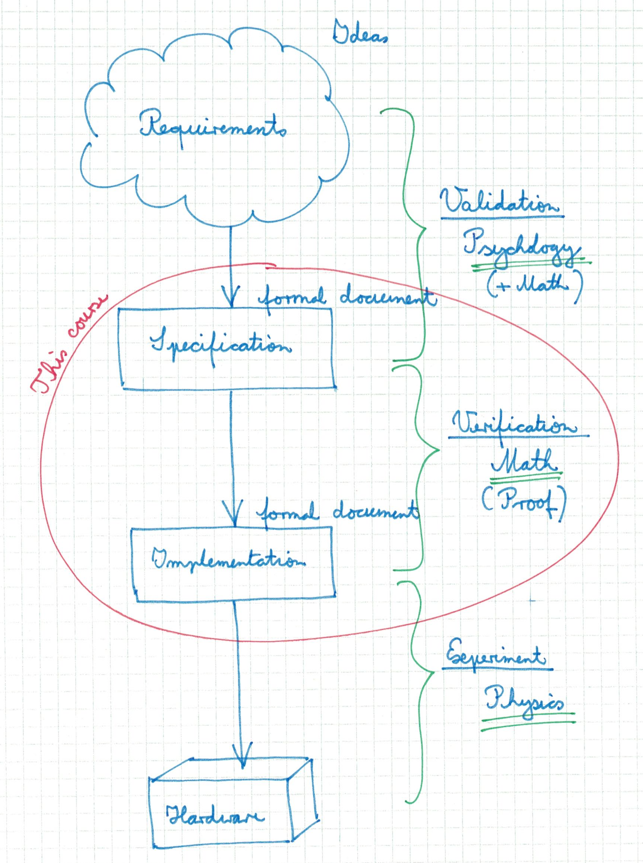
\includegraphics[width=0.5\textwidth]{figures/validationverification.png}
\caption{Validation and Verification}
\end{figure}

Focus on verification:

\begin{itemize}
\tightlist
\item
  Specification and implementation

  \begin{itemize}
  \tightlist
  \item
    two descriptions of the same problem, and that with different points
    of view
  \item
    redundancy
  \end{itemize}
\item
  How to Know Consistency?

  \begin{itemize}
  \tightlist
  \item
    Testing
  \item
    Proving
  \item
    Combination of both
  \end{itemize}
\end{itemize}

\hypertarget{testing}{%
\subsubsection{Testing}\label{testing}}

\begin{itemize}
\tightlist
\item
  program will be executed on chosen input
\item
  is output consistent with specification?

  \begin{itemize}
  \tightlist
  \item
    yes: no (nearly no) knowledge gained
  \item
    no: now we know more: that the program contains an error
  \end{itemize}
\end{itemize}

\begin{tcolorbox}[colback=red!5!white,colframe=red!75!black]
\textbf{Dijkstra's famous statement} \\
"The number of different inputs, i.e. the number of different computations for which the assertions claim to hold is so fantastically high that demonstration of correctness by sampling is completely out of the question. Program testing can be used to show the presence of bugs, but never to show their absence!"
\end{tcolorbox}

In other words: A successful industrial acceptance test does not mean
that a software product is free of errors; it just means that the
customer has to pay

\hypertarget{proving}{%
\subsubsection{Proving}\label{proving}}

\begin{itemize}
\tightlist
\item
  program will not be executed
\item
  rather we try to find a mathematical proof
\item
  do we find a proof?

  \begin{itemize}
  \tightlist
  \item
    yes: now we know that the program is correct
  \item
    no: we know that the program might contain errors, or a good idea
    for the proof is (still) missing
  \end{itemize}
\end{itemize}

\hypertarget{testing-and-proving}{%
\subsubsection{Testing and Proving}\label{testing-and-proving}}

\begin{itemize}
\tightlist
\item
  Testing: good for finding bugs
\item
  Proving: good for showing that there are no bugs
\item
  good practical method:

  \begin{itemize}
  \tightlist
  \item
    first: test your program to find as many errors as possible
  \item
    then: try to prove your program correct
  \end{itemize}
\end{itemize}

\clearpage
\hypertarget{state}{%
\subsection{State}\label{state}}

\begin{itemize}
\tightlist
\item
  the distinguishing feature of any imperative programming language is
  the explicit manipulation of state
\item
  the state of an imperative program can be modelled as a function that
  maps the variables (VAR) of a program to their current contents (VAL):

  \begin{itemize}
  \tightlist
  \item
    STATES = VAR -\textgreater{} VAL
  \item
    $\sigma$1, $\sigma$2, $\sigma$3, $\sigma$4 : STATES
  \end{itemize}
\end{itemize}

\begin{lstlisting}
$\sigma$1(x) = 17, $\sigma$1(y) = 5
x := x - y;
$\sigma$2(x) = 17 - 5 = 12, $\sigma$2(y) = 5
y := x + y;
$\sigma$3(x) = 12, $\sigma$3(y) = 12 + 5 = 17
x := y - x
$\sigma$4(x) = 17 - 12 = 5, $\sigma$4(y) = 17
\end{lstlisting}

\hypertarget{boolean-expressions}{%
\subsection{Boolean Expressions}\label{boolean-expressions}}

\begin{itemize}
\tightlist
\item
  given a boolean expression and a state

  \begin{itemize}
  \tightlist
  \item
    boolean expression either true or false
  \end{itemize}
\item
  condition in if or while command

  \begin{itemize}
  \tightlist
  \item
    condition will be evaluated; yields either true or false
  \end{itemize}
\item
  condition as assert command

  \begin{itemize}
  \tightlist
  \item
    should always yield true; if it does not, the program is in error
  \end{itemize}
\end{itemize}

\hypertarget{assertions}{%
\subsection{Assertions}\label{assertions}}

\begin{itemize}
\tightlist
\item
  in programming languages like Java, the assert commands contain
  boolean expressions that can be evaluated at run time
\item
  in verification languages like IML or Dafny, the assert commands
  contain assertions
\item
  an assertion describes a set of states: the set of all states that
  satisfy the assertion

  \begin{itemize}
  \tightlist
  \item
    the assertion `x \textgreater{} 5' describes the set of all states
    with $\sigma$(x) \textgreater{} 5, for example
  \item
    $\sigma$1 with $\sigma$1(x) = 6 and $\sigma$1(y) = 25, or
  \item
    $\sigma$2 with $\sigma$2(x) = 17 and $\sigma$2(y) = 35
  \item
    the assertion `true' describes the set of all states that satisfy
    true, that is, the full set of all possible states
  \end{itemize}
\end{itemize}

\hypertarget{implication}{%
\subsection{Implication}\label{implication}}

\begin{figure}[H]
\centering
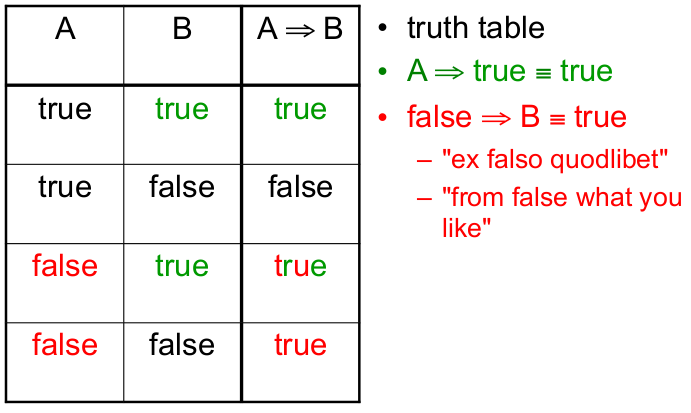
\includegraphics[width=0.5\textwidth]{figures/implication.png}
\caption{Implication}
\end{figure}

\begin{itemize}
\tightlist
\item
  ``If I win, I'll eat my hat.''
\item
  is true

  \begin{itemize}
  \tightlist
  \item
    if I do not win (independent of what I will do with my hat) --- ex
    falso quodlibet
  \item
    if I win and I eat my hat
  \end{itemize}
\item
  is false

  \begin{itemize}
  \tightlist
  \item
    if I win but I do not eat my hat
  \end{itemize}
\end{itemize}

\begin{figure}[H]
\centering
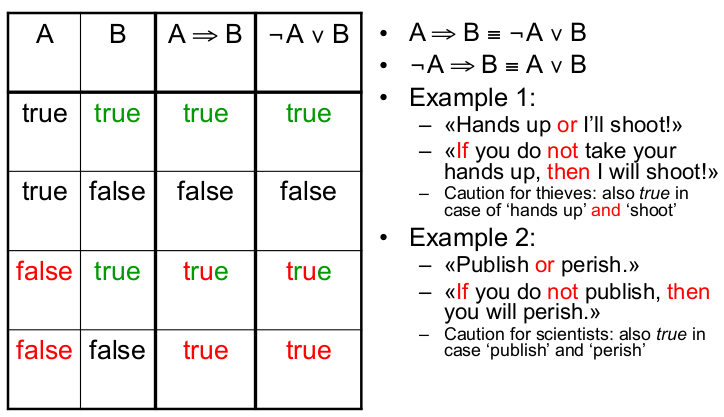
\includegraphics[width=0.7\textwidth]{figures/implication2.png}
\caption{Implication 2}
\end{figure}

\begin{itemize}
\tightlist
\item
  implication has nothing to do with causal relations; just the truth
  table matters
\item
  if A is false, the implication will always be true.
\end{itemize}

\clearpage
\hypertarget{weaker-and-stronger-conditions}{%
\subsubsection{Weaker and Stronger
Conditions}\label{weaker-and-stronger-conditions}}

\begin{itemize}
\tightlist
\item
  examples:

  \begin{itemize}
  \tightlist
  \item
    x = 5 $\land$ y = 7 -\textgreater{} x = 5
  \item
    x = 5 -\textgreater{} x = 5 $\lor$ y = 7
  \end{itemize}
\item
  P -\textgreater{} Q

  \begin{itemize}
  \tightlist
  \item
    P more restrictive than Q
  \item
    set of states given by P is subset of set of states given by Q
  \item
    P stronger than Q
  \item
    Q weaker than P
  \end{itemize}
\item
  boundary cases:

  \begin{itemize}
  \tightlist
  \item
    What is the strongest condition? --\textgreater{} False
  \item
    What is the weakest condition? --\textgreater{} True
  \end{itemize}
\end{itemize}

\hypertarget{validity-versus-truth}{%
\subsubsection{Validity Versus Truth}\label{validity-versus-truth}}

\begin{itemize}
\tightlist
\item
  A boolean formula B (for example an assertion or a Hoare triple) is
  valid if it is true in all states, written $\models$ B.

  \begin{itemize}
  \tightlist
  \item
    x + 5 = 5 + x is true in all states
  \item
    thus x + 5 = 5 + x is valid: $\models$ x + 5 = 5 + x
  \end{itemize}
\end{itemize}

\clearpage
\hypertarget{hoare-triples}{%
\subsection{Hoare Triples}\label{hoare-triples}}

A Hoare triple consists of

\begin{itemize}
\tightlist
\item
  an assertion P, called the \textbf{precondition} of the Hoare triple
\item
  a command C
\item
  an assertion Q, called the \textbf{postcondition} of the Hoare triple
\end{itemize}

\textit{Note: P and Q are the precondition and postcondition of the Hoare
triple, not precondition and postcondition of the command}

\begin{lstlisting}
{ x = 5 } x := x + 1 { x = 17 }
{ x > 5 } x := x + 1 { x > 6 }
{ j = 0 } while i = 0 do skip endwhile { k = 0 }
\end{lstlisting}

\begin{itemize}
\tightlist
\item
  a Hoare triple itself is a boolean formula, which can be true in some
  state and false in others
\item
  we call the state in which execution of C begins the \textbf{prestate}
  of that execution, and the resulting state its \textbf{poststate}, the
  latter provided that execution terminates
\end{itemize}

\begin{tcolorbox}[colback=red!5!white,colframe=red!75!black]
((prestate satisfies P $\wedge$ execution of C terminates) $\Rightarrow$ poststate satisfies Q)
\end{tcolorbox}

\begin{itemize}
\tightlist
\item
  This means, if the prestate is wrong, the full Hoare tripple is true
  (since it's an implication)
\item
  The prestate also includes the termination of the program c. If the
  program doesn't terminate, everything is ok
\end{itemize}

\begin{figure}[H]
\centering
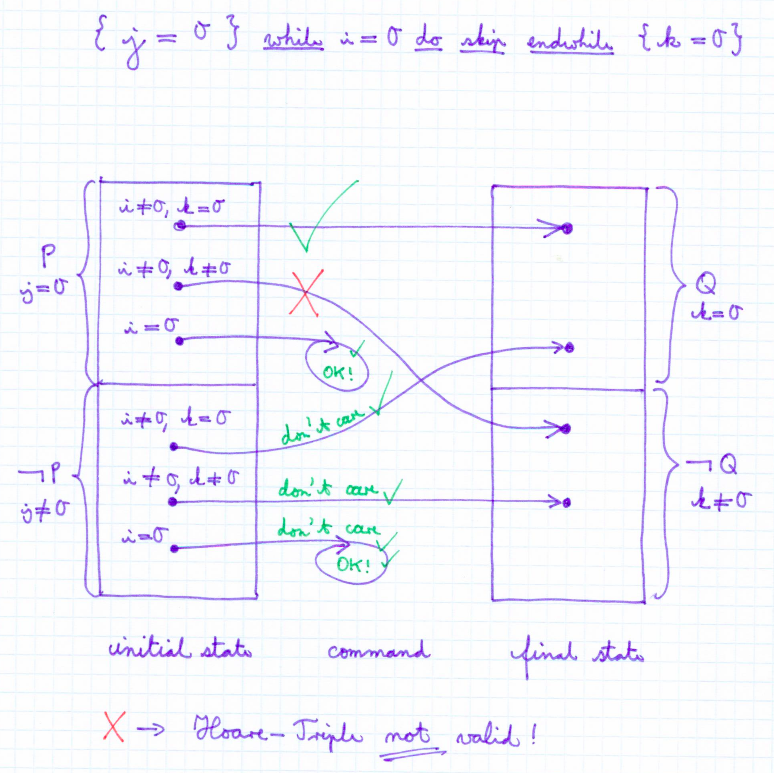
\includegraphics[width=0.6\textwidth]{figures/hoaretriple.png}
\caption{Hoare Triple example}
\end{figure}

\begin{itemize}
\tightlist
\item
  given the following Hoare triple:

  \begin{itemize}
  \tightlist
  \item
    \{ j = 0 \} while i = 0 do skip endwhile \{ k = 0 \}
  \end{itemize}
\item
  The example above describes all 8 kinds of prestates (i = 0 implies 2
  states each).
\item
  The example shows, that the hoare triple would be false in one
  prestate and thus the hoarse triple itself is not valid.
\end{itemize}

\hypertarget{conditional-or-partial-correctness}{%
\subsubsection{Conditional or Partial
Correctness}\label{conditional-or-partial-correctness}}

\begin{itemize}
\tightlist
\item
  A Hoare triple \{P\} C \{Q\} is called \textbf{valid}, written $\models$ \{P\}
  C \{Q\} if it is true in all prestates.
\item
  A Hoare triple is valid, If execution of command C begins in any state
  that satisfies the precondition P and execution terminates, then the
  resulting state satisfies the postcondition Q.
\item
  Note that a valid Hoare triple does not provide any information
  concerning the resulting state if execution begins in any state that
  does not satisfy the precondition.
\item
  We are only interested in valid Hoare triples.
\end{itemize}

\begin{tcolorbox}[colback=red!5!white,colframe=red!75!black]
Examples: \\
– $\nvDash$ { x = 5 } x := x + 1 { x = 17 } (this is not valid, since the postcondition could not be met) \\
– $\models$ { x > 5 } x := x + 1 { x > 6 } \\
– $\nvDash$ { j = 0 } while i = 0 do skip endwhile { k = 0 }
\end{tcolorbox}

\hypertarget{total-vs.partial-correctness}{%
\subsubsection{Total vs.~Partial
Correctness}\label{total-vs.partial-correctness}}

\begin{itemize}
\tightlist
\item
  If the precondition is true, the execution terminates properly and the
  postcondition is true, the Hoare triple is called totally correct.
\item
  If you don't know if the execution terminates properly, but if it
  terminates the result is true, the Hoare triple is called partially
  correct.
\end{itemize}

\hypertarget{specification-of-imperative-programs}{%
\subsection{Specification of Imperative
Programs}\label{specification-of-imperative-programs}}

A specification for imperative programs should provide the following
information:

\begin{itemize}
\tightlist
\item
  a precondition P
\item
  a list x of variables that may be changed

  \begin{itemize}
  \tightlist
  \item
    with the important understanding that all other variables must not
    be changed
  \end{itemize}
\item
  a postcondition Q
\end{itemize}

We denote such a specification by \{P\} x:=? \{Q\}

\hypertarget{specification-for-integer-square-root}{%
\subsubsection{Specification for Integer Square
Root}\label{specification-for-integer-square-root}}

\begin{itemize}
\tightlist
\item
  English spec

  \begin{itemize}
  \tightlist
  \item
    Find an integer approximation to the square root of integer a.
  \end{itemize}
\item
  add precision

  \begin{itemize}
  \tightlist
  \item
    a $\geqslant$ 0
  \item
    store result in variable r
  \item
    choose largest integer r such that $r^2$ $\leqslant$ a
  \end{itemize}
\item
  formal spec

  \begin{itemize}
  \tightlist
  \item $\{0 \leqslant a\} r:=? \{r^2 \leqslant a < (r + 1)^2\}$
  \end{itemize}
\end{itemize}

It is important to list all the variables that are allowed to be changed
(r := ?). If we would not define that, we could change a to 0 to meet
the conditions.

\hypertarget{rigid-variables}{%
\subsubsection{Rigid Variables}\label{rigid-variables}}

Rigid variables can be introduced to connect the pre- and the
postconditions with variables that only occur in assertions and not in
the program.

\{ x = X \} x:=? \{ x = X + 6 \}

this means: for all values X, if x = X in the initial state and
execution terminates, then x = X + 6 in the final state.

\clearpage
\hypertarget{hoare-logic-and-its-mechanization}{%
\section{Hoare Logic and its
Mechanization}\label{hoare-logic-and-its-mechanization}}

\begin{itemize}
\tightlist
\item
  means to prove the Hoare triple \{ P \} C \{ Q \} valid
\item
  Hoare logic is a logic for obtaining valid Hoare triples by purely
  deductive reasoning, that is, by mathematical proof
\item
  deductive reasoning means successively applying inference rules to
  axioms and already obtained conclusions to obtain new conclusions
\item
  such proofs usually are extremely long and boring
\item
  and therefore must be performed as automatically as possible (by
  programs that are by themselves reliable \ldots{})
\item
  but: proof problem is undecidable in the general case
\end{itemize}

\hypertarget{weakest-preconditions}{%
\subsection{Weakest Preconditions}\label{weakest-preconditions}}

\begin{itemize}
\tightlist
\item
  given a command C and a postcondition Q
\item
  given a prestate, the following three things may happen:

  \begin{enumerate}
  \def\labelenumi{\alph{enumi})}
  \tightlist
  \item
    execution of C terminates in a poststate that satisfies Q
  \item
    execution of C does not terminate
  \item
    execution of C terminates in a poststate that satisfies $\neg$Q
  \end{enumerate}
\item
  let w be the set of all prestates from a) and b) together
\item
  a weakest precondition W for C and Q is a boolean formula that
  describes exactly this set
\item
  obviously, weakest preconditions are not unique, since with W $\in$ wp(C,
  Q), for instance, W $\land$ true $\in$ wp(C, Q)
\item
  but clearly, all W $\in$ wp(C, Q) are equivalent
\end{itemize}

\begin{tcolorbox}[colback=red!5!white,colframe=red!75!black]
$\models$ { P } C { Q } is equivalent to $\models$ P $\Rightarrow$ wp(C, Q)
\end{tcolorbox}

\hypertarget{rules-of-inference}{%
\subsection{Rules of Inference}\label{rules-of-inference}}

\begin{itemize}
\tightlist
\item
  let f, f 1 , \ldots{}, f n be boolean formulas (here assertions or
  Hoare triples), n $\geqslant$ 0
\item
  an inference rule is a syntactic construct of the following form:
\end{itemize}

\begin{figure}[H]
\centering
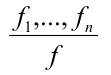
\includegraphics[width=50px]{figures/inferenceRule.png}
\caption{Inference Rule}
\end{figure}

\begin{itemize}
\tightlist
\item
  f\_1 , \ldots{}, f\_n are called premises or hypotheses
\item
  f is called conclusion
\item
  if there are no premises (n = 0), the rule is called an axiom
\item
  the conclusion f is valid, if all hypotheses are valid
\end{itemize}

\hypertarget{skip-axiom}{%
\subsubsection{Skip Axiom}\label{skip-axiom}}

\begin{figure}[H]
\centering
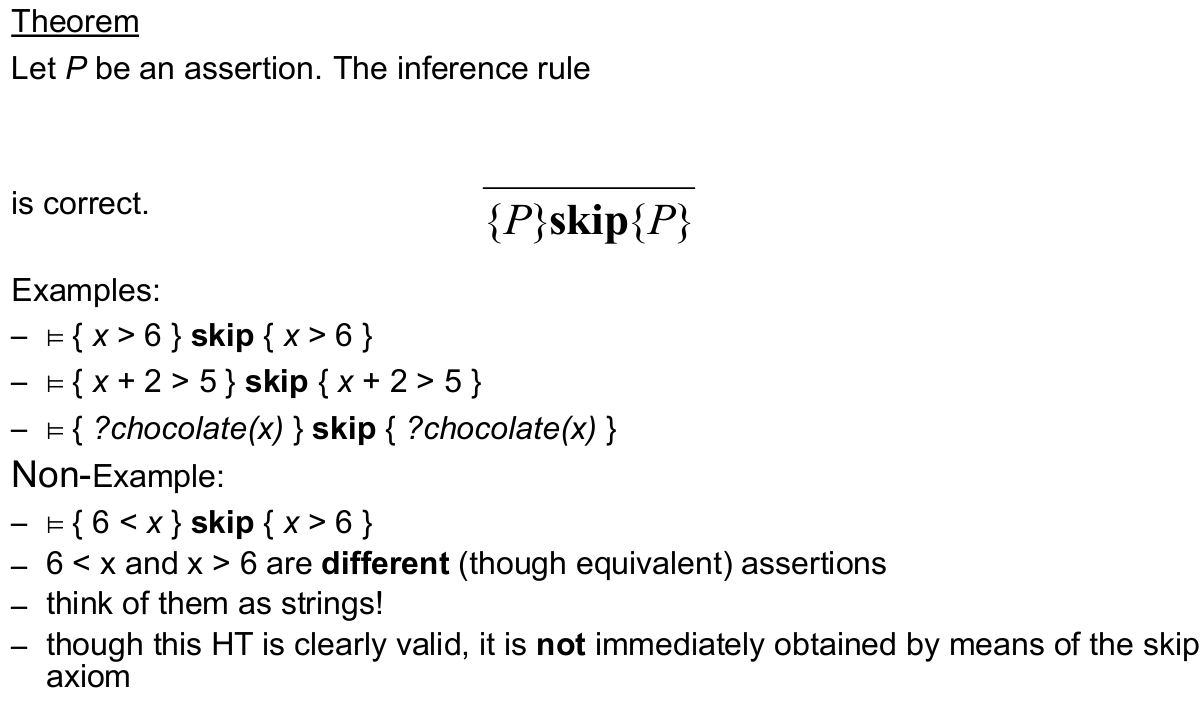
\includegraphics[width=0.7\textwidth]{figures/skipAxiom.png}
\caption{Skip Axiom}
\end{figure}

\begin{tcolorbox}[colback=red!5!white,colframe=red!75!black]
$\{ 6 < x \}$ not equal $\{ x > 6 \}$
\end{tcolorbox}

\clearpage
\hypertarget{rule-of-consequence}{%
\subsection{Rule of Consequence}\label{rule-of-consequence}}

the RoC is of utmost importance:

\begin{itemize}
\tightlist
\item
  it provides the interface between Hoare logic, concerned with
  programming, and „ordinary`` mathematics
\item
  \ldots{} or in other words, it allows to plug in ordinary mathematics
  into Hoare logic
\end{itemize}

\begin{figure}[H]
\centering
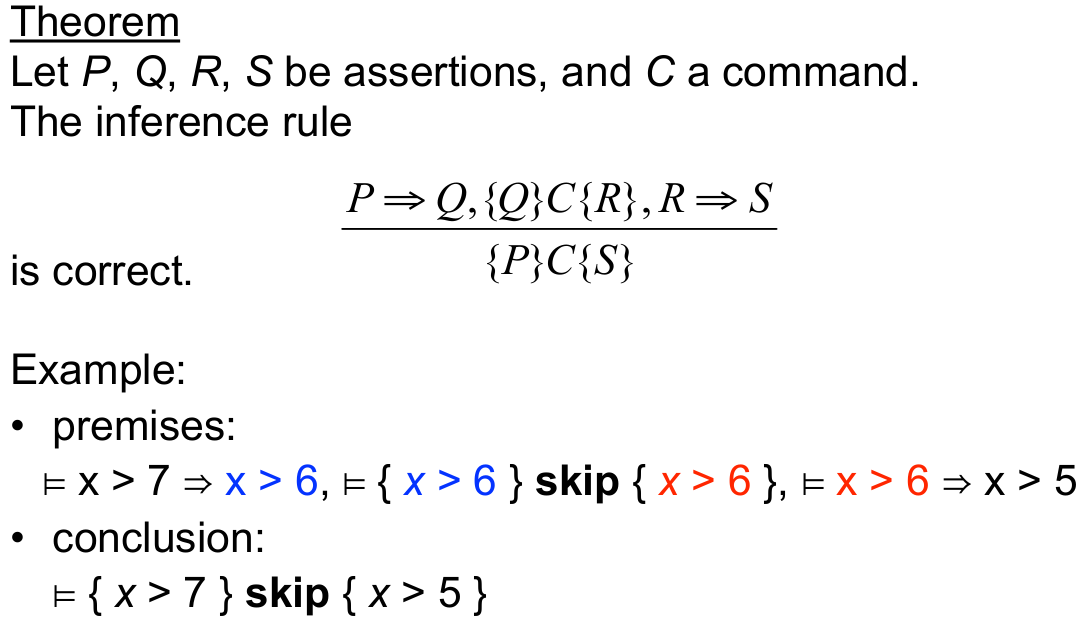
\includegraphics[width=0.7\textwidth]{figures/rulesOfConsquence.png}
\caption{Rules of Consequence}
\end{figure}

We now write this proof of $\models$ \{ x \textgreater{} 7 \} skip \{ x
\textgreater{} 5 \} more concisely and much closer to normal programming
as

\begin{lstlisting}
{ x > 7 }
{ x > 6 }
skip
{ x > 6 }
{ x > 5 }
\end{lstlisting}

\begin{itemize}
\tightlist
\item
  premises:

  \begin{itemize}
  \tightlist
  \item
    we read lines 1 and 2 as implication $\Rightarrow$ (first premise of RoC)
  \item
    we read lines 2 --- 4 as HT (second premise of RoC)
  \item
    we read lines 4 and 5 as implication $\Rightarrow$ (third premise of RoC)
  \end{itemize}
\item
  conclusion:

  \begin{itemize}
  \tightlist
  \item
    we read lines 1 --- 5 as HT (conclusion of RoC)
  \end{itemize}
\end{itemize}

\clearpage
\hypertarget{general-proof-procedure}{%
\subsection{General Proof Procedure}\label{general-proof-procedure}}

\begin{itemize}
\tightlist
\item
  To prove \{P\} C \{Q\}, we start with the postcondition Q, go
  backwards over the command C to determine a precondition R such that
  the HT \{R\} C \{Q\} is valid, and construct the implication P
  -\textgreater{} R.
\item
  This implication is called a verification condition (VC).
\item
  If this VC is valid, then the original HT \{P\} C \{Q\} is valid too.
\item
  this process can be mechanized, that is, performed fully automatically
  be means of a - computer
\item
  there might be many possible preconditions, which one do we choose?
\item
  we always choose the syntactically weakest precondition
\item
  that is, we can assume as little as possible
\end{itemize}

\begin{lstlisting}
Example
{ x > 7 } -- given precondition P
{ x > 5 } -- compute precondition R
skip  
-- go backwards over the command C
{ x > 5 } -- start here with given postcondition Q now construct VC P $\Rightarrow$ R, 
          -- that is, "x > 7 $\Rightarrow$ x > 5"
\end{lstlisting}

\hypertarget{computing-preconditions-and-software-engineering}{%
\subsubsection{Computing Preconditions and Software
Engineering}\label{computing-preconditions-and-software-engineering}}

\begin{itemize}
\tightlist
\item
  looks strange in the first moment to start with the postcondition to
  arrive at the precondition
\item
  but: \textbf{the postcondition describes the actual task of the
  program and is thus given}
\item
  the precondition will be determined to find out under which
  circumstances the postcondition can be achieved
\item
  happily, determining preconditions from postconditions is much simpler
  than the other way round
\item
  thus, determining VCs (via computing preconditions) can be done
  automatically by a tool called a \textbf{verification condition
  generator}
\item
  the VCs can then (hopefully automatically) be discharged (proved
  valid) by a second tool called a theorem prover
\end{itemize}

\hypertarget{textual-substitution}{%
\subsubsection{Textual Substitution}\label{textual-substitution}}

This is an operation that essentially can be performed by means of
search and replace of a text editor, and thus can be implemented on a
machine.

\begin{lstlisting}
x[x<-z+2] yields (z + 2)
-- or
y[x<-z+2] yields y
-- [x<-z+2] this will replace all x with z+2
\end{lstlisting}

\hypertarget{assignment-axiom}{%
\subsection{Assignment Axiom}\label{assignment-axiom}}

\begin{itemize}
\tightlist
\item
  The assigning command can be seen as something like renaming an
  expression in the precondition.
\item
  You take the expression in the execution part and assign this defition
  of the variable (in the execution part) to the same variable in the
  precondition.
\item
  If the new precondition can still meet the postcondition (after
  execution), the Hoare is valid.
\end{itemize}

\begin{figure}[H]
\centering
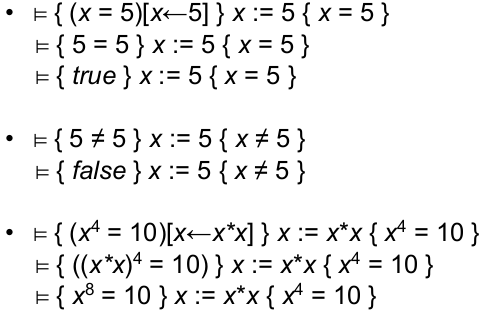
\includegraphics[width=0.5\textwidth]{figures/assigningAxiom.png}
\caption{Assignment Axiom Examples}
\end{figure}

\hypertarget{composition-command}{%
\subsection{Composition Command}\label{composition-command}}

The composition command is used to do one or more things one after the
other.

\begin{figure}[H]
\centering
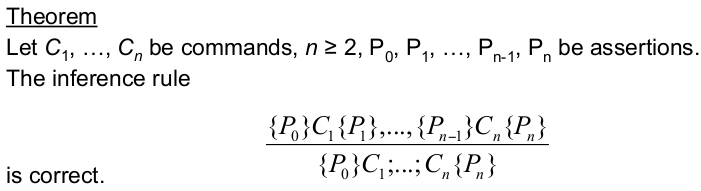
\includegraphics[width=0.7\textwidth]{figures/compositionrule.png}
\caption{Composition Rule}
\end{figure}

\begin{figure}[H]
\centering
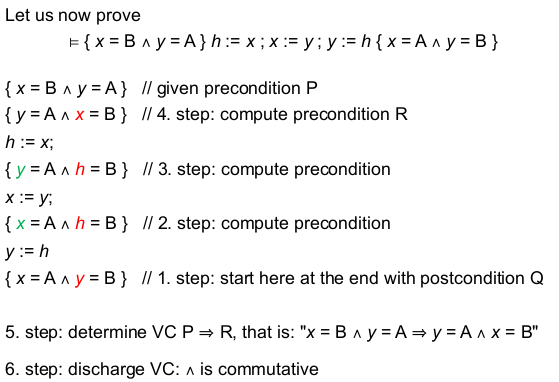
\includegraphics[width=0.5\textwidth]{figures/compositionExample.png}
\caption{Composition Example}
\end{figure}

\hypertarget{example-strange-swap}{%
\subsubsection{Example Strange Swap}\label{example-strange-swap}}

\begin{figure}[H]
\centering
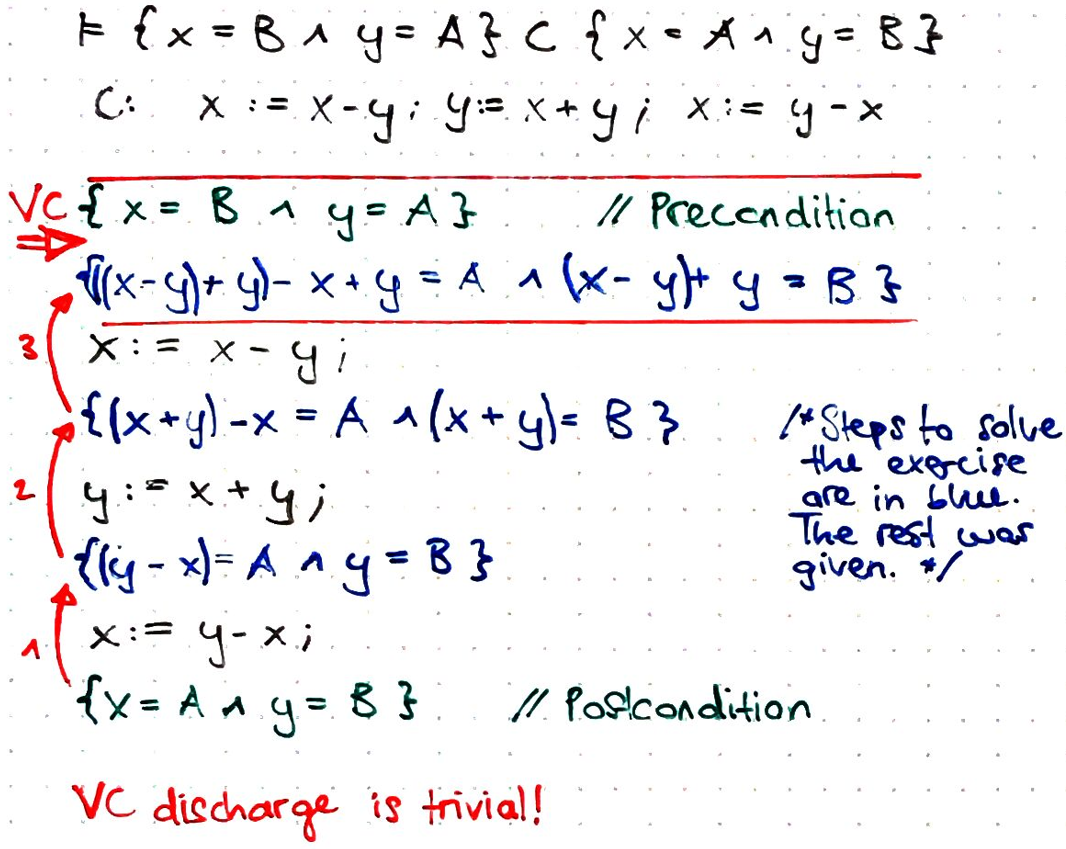
\includegraphics[width=0.6\textwidth]{figures/exampleStrangeSwap.png}
\caption{Strange Swap Example}
\end{figure}

\hypertarget{conditional-rule}{%
\subsection{Conditional Rule}\label{conditional-rule}}

\begin{figure}[H]
\centering
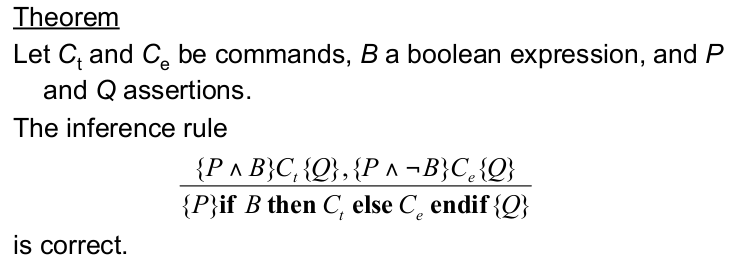
\includegraphics[width=0.6\textwidth]{figures/conditionalRule.png}
\caption{Conditional Rule}
\end{figure}

\begin{figure}[H]
\centering
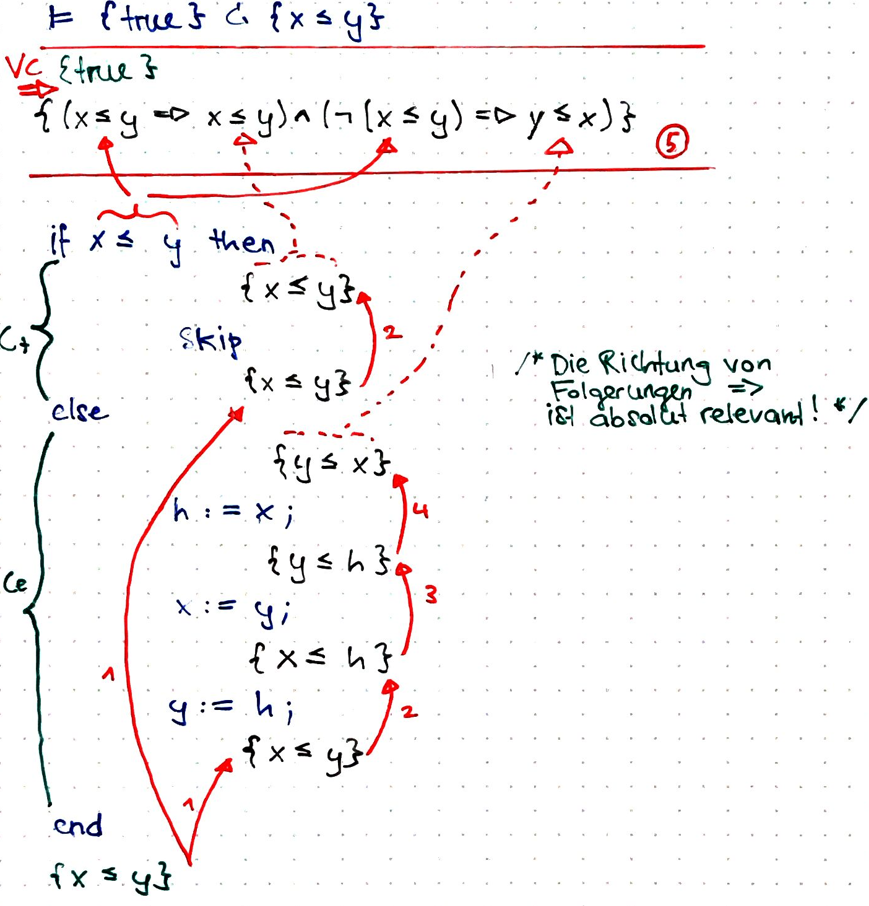
\includegraphics[width=0.8\textwidth]{figures/exampleConditional.png}
\caption{Conditional Rule Example}
\end{figure}

\clearpage
\hypertarget{loops-and-invariants}{%
\section{Loops and Invariants}\label{loops-and-invariants}}

\hypertarget{invariants}{%
\subsection{Invariants}\label{invariants}}

An assertion I is called an invariant, if a command C doesn't change
anything in regards to the assertion I. -\textgreater{} $\models$ \{ I \} C \{ I
\}

E.g. if you drive through a tunnel by car, you pass an emergency exit
every 250 meters. If you are between two exits and you are driving
forward, you are maximizing the distance to the earlier exit and
minimizing the distance to the next exit, but you don't change the
distance between them. The distance between them is invariant.

\hypertarget{invariants-for-loops}{%
\subsubsection{Invariants for loops}\label{invariants-for-loops}}

\begin{itemize}
\tightlist
\item
  here we need invariants for loops
\item
  but at the beginning of the loop body we can assume more than the
  invariant only: we can also assume the loop condition
\end{itemize}

\begin{lstlisting}
while i > 0 do
    { i >= 0 $\land$ i > 0 } --invariant $\land$ condition
    { (i - 1) >= 0 }
    i := i - 1
    { i >= 0 } --invariant
endwhile
\end{lstlisting}

\begin{itemize}
\tightlist
\item
  an invariant I of the body C relative to the condition B of a loop
  indeed is an invariant of the complete loop
\end{itemize}

\begin{lstlisting}
{ I }
while B do
    { I $\land$ B }
    C
    { I }
endwhile
{ I }
\end{lstlisting}

\begin{figure}[H]
\centering
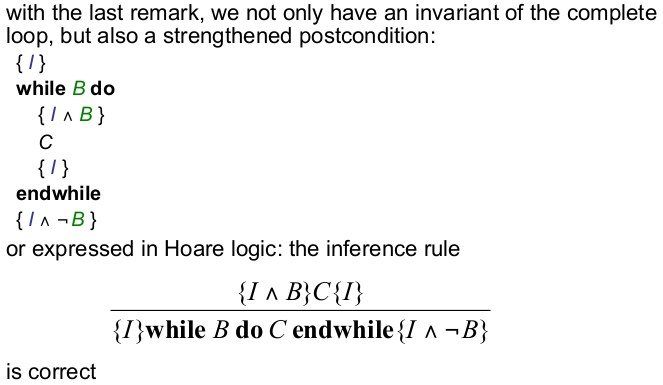
\includegraphics[width=0.7\textwidth]{figures/invariantLoop.png}
\caption{Invariants of a Loop}
\end{figure}

\hypertarget{finding-invariants}{%
\subsubsection{Finding Invariants}\label{finding-invariants}}

\begin{itemize}
\tightlist
\item
  to find an appropriate invariant is a creative process, just like
  programming
\item
  it cannot be automated
\item
  however, after having found an invariant, it can be added as
  annotation to the loop
\item
  and then, the generation of verification conditions can again be
  performed fully automatically
\end{itemize}

\clearpage
\hypertarget{scala}{%
\section{Scala - Introduction}\label{scala}}

\begin{itemize}
\tightlist
\item
  Multi-paradigm Programming

  \begin{itemize}
  \tightlist
  \item
    A multi-paradigm programming language provides ``a framework in
    which programmers can work in a variety of styles, freely
    intermixing constructs from different paradigms.''
  \end{itemize}
\end{itemize}

\begin{figure}[H]
\centering
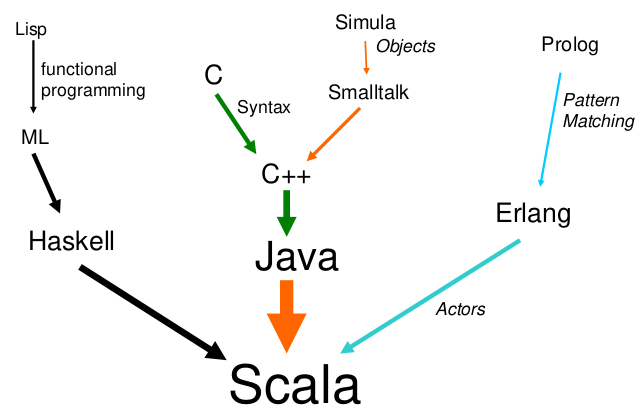
\includegraphics[width=0.7\textwidth]{figures/scalaOverview.png}
\caption{Scala Overview}
\end{figure}

Scala is

\begin{itemize}
\tightlist
\item
  Object-Oriented
\item
  Functional
\item
  Safe and performant, with strong static typing
\item
  Agile, with lightweight syntax
\item
  Scalable
\item
  Extensible
\end{itemize}

\clearpage
\hypertarget{scala-advantages-over-java}{%
\subsection{Scala Advantages over
Java}\label{scala-advantages-over-java}}

\begin{itemize}
\tightlist
\item
  In Scala functions are first class and can be passed around

  \begin{itemize}
  \tightlist
  \item
    This encourages functional programming with all its advantages
    (=\textgreater{} Java8)
  \end{itemize}
\item
  In Scala all values are objects (pure object-oriented)

  \begin{itemize}
  \tightlist
  \item
    The compiler turns them into primitives, so no efficiency is lost
  \end{itemize}
\item
  In Scala operators are just methods

  \begin{itemize}
  \tightlist
  \item
    a * b \textless{}-\textgreater{} a.*(b)
  \end{itemize}
\item
  Scala is statically typed (as Java) but uses type inference

  \begin{itemize}
  \tightlist
  \item
    val m = HashMap{[}String,List{[}String{]}{]}()(=\textgreater{}
    Java10 var)
  \end{itemize}
\item
  Scala supports the principle of uniform access

  \begin{itemize}
  \tightlist
  \item
    A field defined as attribute or as method is accessed uniformly
  \end{itemize}
\item
  Scala supports concurrency

  \begin{itemize}
  \tightlist
  \item
    Actor Library for coarse-grained concurrency
  \item
    Immutable data structures =\textgreater{} avoids race conditions
  \end{itemize}
\end{itemize}

\hypertarget{getting-started}{%
\subsection{Getting started}\label{getting-started}}

\hypertarget{compiling}{%
\subsubsection{Compiling}\label{compiling}}

\begin{lstlisting}[language=scala]
>scalac HelloWorld.scala

>scala HelloWorld
Hello world!
>scala -cp . HelloWorld
Hello world!
\end{lstlisting}

\hypertarget{scala-code-may-use-any-java-class}{%
\subsubsection{Scala Code may use any Java
class}\label{scala-code-may-use-any-java-class}}

\begin{lstlisting}[language=scala]
import javax.swing._
import java.awt._

object SampleGUI {
    def main(args: Array[String]) {
        val f = new JFrame("Title")
        f.setLayout(new FlowLayout())
        f.add(new JLabel("text"))
        f.add(new JButton("OK"))
        f.pack
        f.setVisible(true)
    }
}
\end{lstlisting}

\hypertarget{types}{%
\subsection{Types}\label{types}}

\begin{itemize}
\tightlist
\item
  Byte, Short, Int, Long, Float, Double

  \begin{itemize}
  \tightlist
  \item
    have methods
  \item
    Operators are method calls
  \item
    Assignment compatibility: Byte -\textgreater{} Short -\textgreater{}
    Int -\textgreater{} Long -\textgreater{} Float -\textgreater{}
    Double
  \end{itemize}
\item
  Char

  \begin{itemize}
  \tightlist
  \item
    Assignment compatibility: Char -\textgreater{} Int
  \end{itemize}
\item
  Boolean
\item
  String

  \begin{itemize}
  \tightlist
  \item
    More methods as in Java:
  \item
    String interpolation
  \item
    Multiline Strings
  \end{itemize}
\item
  Unit
\end{itemize}

\begin{figure}[H]
\centering
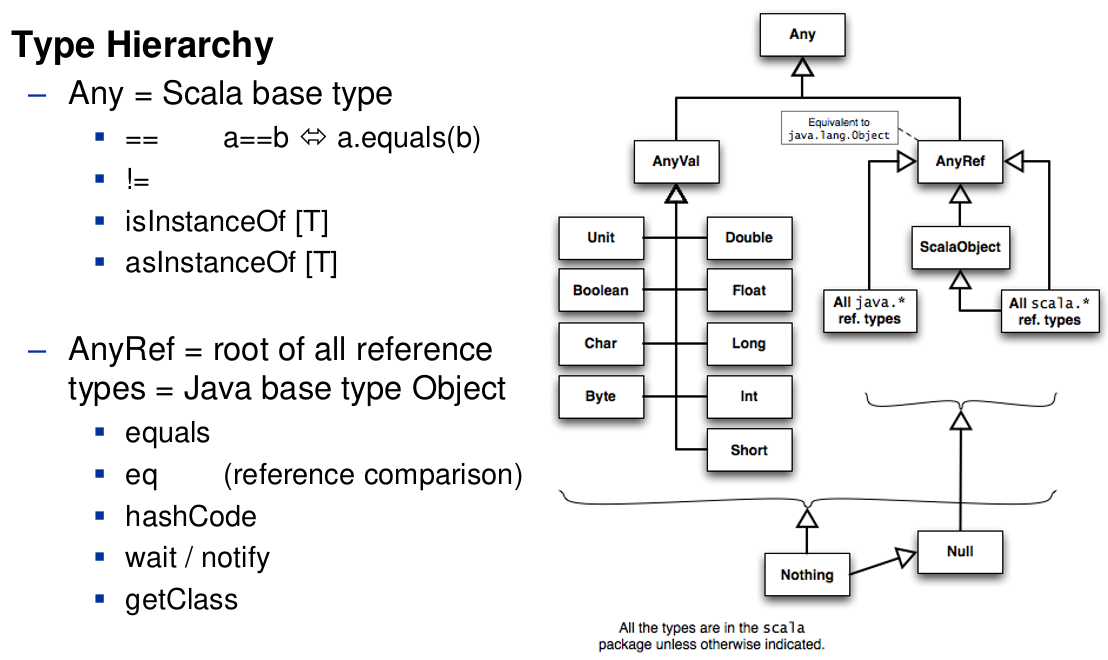
\includegraphics[width=0.9\textwidth]{figures/scalaTypes.png}
\caption{Scala Types}
\end{figure}

\clearpage
\begin{itemize}
\tightlist
\item
  Unit

  \begin{itemize}
  \tightlist
  \item
    Corresponds to \textbf{void in Java}, is used as result type for
    ``procedures''
  \item
    Unit type has only one value: ()
  \end{itemize}
\item
  Null

  \begin{itemize}
  \tightlist
  \item
    Subtype of all reference types
  \item
    Its only instance is null
  \end{itemize}
\item
  Nothing

  \begin{itemize}
  \tightlist
  \item
    Bottom type, is a subtype of all types
  \end{itemize}
\end{itemize}

\hypertarget{lists}{%
\subsubsection{Lists}\label{lists}}

\begin{itemize}
\tightlist
\item
  Lists are concrete classes, no interfaces
\item
  A list is implemented as linked list and may contain an arbitrary
  number of elements
\item
  \textbf{Lists are immutable} (mutable variants exist)
\item
  The datatypes are automatically recognized
\end{itemize}

\begin{lstlisting}[language=scala]
scala> val list = List("Hello", "World", "!")
list: List[java.lang.String] = List(Hello, World, !)
scala> list.head
res1: java.lang.String = Hello
scala> list.tail
res2: List[java.lang.String] = List(World, !)
scala> list(2)
res3: java.lang.String = !
scala> 1 :: 2 :: 3 :: Nil
res4: List[Int] = List(1, 2, 3)
\end{lstlisting}

\hypertarget{maps}{%
\subsubsection{Maps}\label{maps}}

\begin{itemize}
\tightlist
\item
  Map contains pairs
\item
  \textbf{Immutable} (mutable variants exist)
\end{itemize}

\begin{lstlisting}[language=scala]
scala> var m = Map("Romeo" -> 22, ("Julia", 21))
m: scala.collection.immutable.Map[String,Int] = Map(Romeo -> 22, Julia -> 21)
scala> m("Romeo")
res1: Int = 22
scala> m = m.updated("Romeo", 25)
m: scala.collection.immutable.Map[String,Int] = Map(Romeo -> 25, Julia -> 21)
scala> m += ("Meier" -> 33)
scala> m
res2: scala.collection.immutable.Map[String,Int] = Map(Romeo -> 25, Julia -> 21, Meier -> 33)
\end{lstlisting}

\hypertarget{variables}{%
\subsubsection{Variables}\label{variables}}

\begin{itemize}
\tightlist
\item
  val

  \begin{itemize}
  \tightlist
  \item
    value, cannot be changed (corresponds to Java's final)
  \end{itemize}
\item
  var

  \begin{itemize}
  \tightlist
  \item
    variable, can be reassigned
  \end{itemize}
\item
  Type declaration is optional upon definition
\end{itemize}

\begin{lstlisting}[language=scala]
scala> val age = 3
age: Int = 3
scala> age = 4 //error: reassignment to val
scala> var age = 34
age: Int = 34
scala> age = 35
age: Int = 35
\end{lstlisting}

\hypertarget{control-expressions}{%
\subsection{Control Expressions}\label{control-expressions}}

\hypertarget{if}{%
\subsubsection{If}\label{if}}

\begin{itemize}
\tightlist
\item
  ``if'' ``('' BooleanExpr ``)'' Expr {[}``else'' Expr{]}
\item
  If-expression returns a result (and has a type!)
\item
  No ternary ``cond ? expr1 : expr2'' operator in Scala
\item
  Expr may be a block expressions
\item
  Type of if expression is ``greatest common base type'' (may be Any)
\end{itemize}

\begin{lstlisting}[language=scala]
scala> val (a,b) = (1,2)
a: Int = 1
b: Int = 2
scala> val max = if(a > b) a else {b}
max: Int = 2
\end{lstlisting}

\hypertarget{loop}{%
\subsubsection{Loop}\label{loop}}

\begin{itemize}
\tightlist
\item
  ``while'' ``('' BooleanExpr ``)'' Expr

  \begin{itemize}
  \tightlist
  \item
    is an expression of type Unit
  \end{itemize}
\item
  ``do'' Expr while ``('' BooleanExpr ``)''

  \begin{itemize}
  \tightlist
  \item
    is an expression of type Unit
  \end{itemize}
\end{itemize}

\hypertarget{for}{%
\subsubsection{For}\label{for}}

\begin{itemize}
\tightlist
\item
  ``for'' ``('' Generators``)'' {[}``yield''{]} Expr
\item
  without yield: is an expression of type Unit
\item
  with yield: is an expression of the type of the first Generator
  (approx.)
\end{itemize}

\begin{lstlisting}[language=scala]
scala> for(i <- 1 to 4) { print(" " + i) }
1 2 3 4
scala> for(i <- List(1,2)) { println(i) }
1
2
scala> val q = for(i <- 1 to 10 if i%2==0) yield (i*i)
q: scala.collection.immutable.IndexedSeq[Int] = Vector(4, 16, 36, 64, 100)
scala> for(i <-1 to 8 by 2; j <- 1 until i) print(i,j)
(3,1)(3,2)(5,1)(5,2)(5,3)(5,4)(7,1)(7,2)(7,3)(7,4)(7,5)(7,6)
\end{lstlisting}

\hypertarget{classes}{%
\subsection{Classes}\label{classes}}

\begin{itemize}
\tightlist
\item
  Object model of Scala is similar to Java's one

  \begin{itemize}
  \tightlist
  \item
    Abstract and final classes
  \item
    Single inheritance of classes
  \item
    Classes may be nested
  \end{itemize}
\item
  Members

  \begin{itemize}
  \tightlist
  \item
    Values (var / val)
  \item
    Methods (def)
  \item
    Types (type)

    \begin{itemize}
    \tightlist
    \item
      In an abstract class, all these members may be abstract (also
      types)!
    \item
      Default visibility is public
    \end{itemize}
  \end{itemize}
\item
  Every class has a primary constructor which is always called

  \begin{itemize}
  \tightlist
  \item
    Auxiliary constructors may be defined
  \end{itemize}
\end{itemize}

\begin{lstlisting}[language=scala]
class CreditCard(val number: Int, var limit: Int) {
    def this(number: Int) = this(number, 1000) // aux constrctor
    println("new card created") // executed in primary constructor
    private var sum = 0
    def buy(amount: Int) {
        if(sum + amount > limit) throw new RuntimeException
        sum += amount
    }
    def remainder = limit-sum // method which does not take parameters
}
\end{lstlisting}

\hypertarget{methods}{%
\subsubsection{Methods}\label{methods}}

\begin{itemize}
\tightlist
\item
  ``def'' id ``('' ParameterList ``)'' {[}``:'' Type{]} = Expr
\item
  Expr may be a single expression or a block expression
\item
  Result of method call is

  \begin{itemize}
  \tightlist
  \item
    Value of expression or
  \item
    Value of argument of a return statement
  \end{itemize}
\item
  If block contains a return statement, then result type must be
  specified
\item
  If method is defined recursively, then result type must be specified
\end{itemize}

\begin{lstlisting}[language=scala]
def add(x: Int, y: Int): Int = {return x+y}
def add(x: Int, y: Int): Int = return x+y
def add(x: Int, y: Int) = x + y
def add(x: Int, y: Int) = { val z = x; z+y }

def max(x: Int, y: Int) = if(x>y) x else y
def fact(x: Int): Int = if(x==0) 1 else x * fact(x-1)
\end{lstlisting}

Parameters may have default values

\begin{lstlisting}[language=scala]
def add(m: Int, n: Int = 1) = m + n
\end{lstlisting}

Parameter may be called by name; named args must follow positional args

\begin{lstlisting}[language=scala]
scala> quorem(n = 2, m = 4)
res1: (Int, Int) = (2,0)
\end{lstlisting}

Parameter lists may be separated (curried)

\begin{lstlisting}[language=scala]
def add(m: Int)(n: Int) = m+n
\end{lstlisting}

\hypertarget{inheritance}{%
\subsubsection{Inheritance}\label{inheritance}}

\begin{lstlisting}[language=scala]
abstract class Base(param: String) {
    def doSomething: String // without body abstract
    val value = param.toInt
    override def toString() = { "^" + super.toString() }
}

class Derived extends Base("0") {
    def doSomething = "working" // override may be added
    override val value = 20
}
\end{lstlisting}

\clearpage
\hypertarget{singleton-objects}{%
\subsubsection{Singleton Objects}\label{singleton-objects}}

The expression \texttt{object} defines automatically a singleton object,
which could be called under it's name.

\begin{lstlisting}[language=scala]
class Color(val r: Int, val g: Int, val b: Int)

object ColorFactory {
    private val cols = Map(
        "red" -> new Color(255,0,0),
        "blue" -> new Color(0,0,255),
        "green" -> new Color(0,255,0))
    def getColor(color: String) =
        if(cols contains color) cols(color) else null
}

scala> ColorFactory.getColor("red")
res0: Color = Color@1e3d24a
scala> ColorFactory.getColor("pink")
res1: Color = null
\end{lstlisting}

\hypertarget{companion-objects}{%
\subsubsection{Companion Objects}\label{companion-objects}}

\begin{itemize}
\tightlist
\item
  Classes and companion objects have no boundaries, they can access the
  private fields and methods of each other
\item
  In the below example the constructor of Color is private, i.e.~new
  instances can only be accessed using method getColor
\end{itemize}

\begin{lstlisting}[language=scala]
class Color private (val r: Int, val g: Int, val b: Int)

object Color {
    private val cols = Map(
        "red" -> new Color(255,0,0),
        "blue" -> new Color(0,0,255),
        "green" -> new Color(0,255,0))

    def getColor(color: String) = if(cols contains color) cols(color) else null

    def apply(color: String) = if(cols contains color) cols(color) else null
}

scala> Color("red")
res0: Color = Color@1623820
scala> Color("pink")
res1: Color = null
\end{lstlisting}

\clearpage
\hypertarget{functions}{%
\subsection{Functions}\label{functions}}

Functions are first-class citizens

\begin{lstlisting}[language=scala,mathescape=false]
scala> val add = (m: Int, n: Int) => m+n
add: (Int, Int) => Int = $$Lambda$1012/2143233788@4962b41e

scala> add(2,3)
res0: Int = 5
\end{lstlisting}

Functions are instances of class FunctionX

\begin{lstlisting}[language=scala,mathescape=false]
scala> val add = (m: Int, n: Int) => m + n
add: (Int, Int) => Int = $$Lambda$1022/196340990@5ec88f9
scala> add.apply(1, 3) // same as add(1,3)
res1: Int = 4
scala> val addc = add.curried
addc: Int => (Int => Int) = scala.Function2$$Lambda@1086
scala> val inc = addc(1)
inc: Int => Int = scala.Function2$$Lambda$1083/2010@11abd6c
scala> inc(5)
res2: Int = 6
scala> val addt = add.tupled
addt: ((Int, Int)) => Int = scala.Function2$$Lambda@219
scala> addt( 1 -> 2)
res3: Int = 3
\end{lstlisting}

\hypertarget{curried}{%
\subsubsection{Curried}\label{curried}}

\begin{lstlisting}[language=scala,mathescape=false]
scala> val add = (x: Int) => (y : Int) => x+y
add: Int => (Int => Int) = $$Lambda$1105/828629051@6aa18912
scala> add(1)
res1: Int => Int = $$Lambda$1106/2034790200@7b364f47
scala> add(1)(2)
res2: Int = 3
\end{lstlisting}

\begin{lstlisting}[language=scala,mathescape=false]
scala> val x = new X()
x: X = X@196a21e
scala> x.add(5)(7)
res0: Int = 12
scala> x.add(5)_
res1: Int => Int = $$Lambda$1135/1230346437@6e4ac3f5
scala> res1(2)
res2: Int = 7
scala> x.add _
res3: Int => (Int => Int) = $$Lambda$1153/855914030@78b293a
\end{lstlisting}

\hypertarget{pattern-matching}{%
\subsection{Pattern Matching}\label{pattern-matching}}

Expr ``match'' ``\{'' CaseClauses ``\}''

\begin{itemize}
\tightlist
\item
  No fall-through
\item
  case \_ is default pattern
\item
  Match throws an error if no pattern matches
\end{itemize}

.

\begin{lstlisting}[language=scala]
def patternMatching(i : Int) = {
    i match {
        case 0 => "Null"
        case 1 => "One"
        case _ => "?"
    }
}
\end{lstlisting}

\hypertarget{matching-lists}{%
\subsubsection{Matching Lists}\label{matching-lists}}

\begin{lstlisting}[language=scala]
def length(list: List[Any]) : Int = {
    list match {
        case List() => 0
        case x :: xs => 1 + length(xs)
    }
}
\end{lstlisting}

\hypertarget{matching-tuples}{%
\subsubsection{Matching Tuples}\label{matching-tuples}}

\begin{lstlisting}[language=scala]
def process(input: Any) = {
    input match {
        case (a,b) => printf("Processing (%d,%d)...\n", a, b)
        case "done" => println("done")
        case _ => null
    }
}
\end{lstlisting}

\hypertarget{case-classes}{%
\subsubsection{Case Classes}\label{case-classes}}

\begin{itemize}
\tightlist
\item
  The new keyword is not mandatory to create instances of these classes
\item
  Getter functions are automatically defined for the constructor
  parameters
\item
  Default definitions for methods equals and hashCode are provided
\item
  Default definition for method toString is provided
\item
  Instances of these classes can be decomposed through pattern matching
\end{itemize}

.

\begin{lstlisting}[language=scala]
abstract class Tree
case class Sum(x: Tree, y: Tree) extends Tree
case class Prod(x: Tree, y: Tree) extends Tree
case class Var(n: String) extends Tree
case class Const(v: Int) extends Tree

def eval(t: Tree, env: Map[String,Int]) : Int = t match {
    case Sum(x, y) => eval(x, env) + eval(y, env)
    case Prod(x, y) => eval(x, env) * eval(y, env)
    case Var(n) => env(n)
    case Const(v) => v
}

scala> val t = Sum(Sum(Var("x"),Var("x")), Prod(Const(7),Var("y")))
t: Sum = Sum(Sum(Var(x),Var(x)),Prod(Const(7),Var(y)))
scala> eval(t, Map("x"->8, "y"->3))
res0: Int = 37
\end{lstlisting}

\clearpage
\hypertarget{scala-traits-eigenschaften}{%
\section{Scala - Traits (Eigenschaften)}\label{scala-traits-eigenschaften}}

\hypertarget{multiple-inheritance}{%
\subsection{Multiple Inheritance}\label{multiple-inheritance}}

Multiple inheritance works fine when you combine classes that have
nothing in common, but there is a conflict if these classes have common
attributes or methods.

\begin{lstlisting}[language=scala,mathescape=false]
class Student { def id: String = ... }
class Employee { def id: String = ... }
class MSEPartTimeStudent extends Student, Employee { ... }
\end{lstlisting}

\hypertarget{problem-of-name-clashes}{%
\subsubsection{Problem of name clashes}\label{problem-of-name-clashes}}

If you have different methods with the same name, but different meaning,
you will also have a conflict in Java. C\# is able to solve this by
defining the class from which the method is derived.\\
\textit{draw from the cowboy means ``ziehen'' in the meaning of draw his
revolver.}

\begin{figure}[H]
\centering
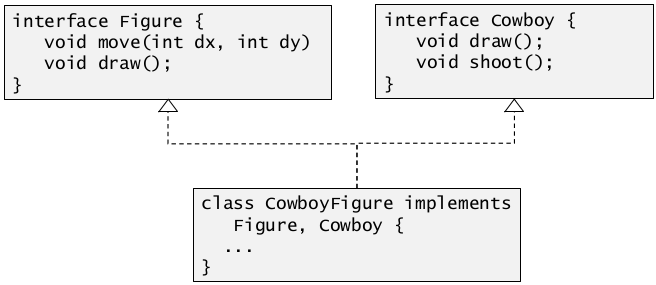
\includegraphics[width=0.7\textwidth]{figures/nameClash.png}
\caption{Name clashes}
\end{figure}

This is even more complicated if the methods are not abstract, but they
have content and inherit different different content.

\begin{lstlisting}[language=scala,mathescape=false]
public interface B {
    default int getValue() { return 1; }
}
public interface C {
    default int getValue() { return 2; }
}
public class D implements B, C {
    public int getValue() {
        return C.super.getValue();
    }
}
\end{lstlisting}

To avoid conflicts, the class D needs to override the method
\texttt{getValue()} and call the method of the mother class.

\clearpage
\hypertarget{example-in-c}{%
\subsubsection{Example in C}\label{example-in-c}}

\begin{lstlisting}[language=C++,mathescape=false]
class A {
    public: int id;
    public: A() { id = 0; }
};
class B1 : public A {
    public: B1() { id = 1; }
};
class B2 : public A {
    public: B2() { id = 2; }
}
class C : public B1, public B2 {};
    static int main(void*) {
    C* c = new C();
    cout << dynamic_cast<B1*>(c) -> id << endl;
    cout << dynamic_cast<B2*>(c) -> id << endl;
    return 0;
}
\end{lstlisting}

This example shows the multiple inheritance from C. In C, the full
content of the classes which I inherit from is copied to the target
class. So if I inherit from two classes, I have two full content of
these two classes. With this behaviour, the code above prints 0012
(because of the dynamic binding).

\hypertarget{java-solution-from-java}{%
\subsubsection{Java solution from Java}\label{java-solution-from-java}}

\begin{itemize}
\tightlist
\item
  Single implementation inheritance
\item
  Multiple interface inheritance

  \begin{itemize}
  \tightlist
  \item
    No solution to the naming problem: If two interfaces introduce
    methods with the same name and signature but of different return
    type, then no class can simultaneously implement both interfaces
  \item
    Inherited default implementation must be resolved explicitly
  \end{itemize}
\end{itemize}

\hypertarget{traits-in-scala}{%
\subsection{Traits in Scala}\label{traits-in-scala}}

Scala traits provide a mixin composition mechanism that has been missing
in Java. Roughly speaking, you can think of traits as analogous to Java
interfaces, but with implementations and fields and dynamic composition.

Traits can be seen as a solution to the

\begin{itemize}
\tightlist
\item
  Diamond problem or
\item
  Linearization Problem
\end{itemize}

\begin{figure}[H]
\centering
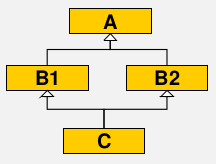
\includegraphics[width=110px]{figures/diamondProblem.png}
\caption{Diamond Problem}
\end{figure}

\begin{itemize}
\tightlist
\item
  Traits encapsulate method and field definitions
\item
  Traits can be reused by mixing them into classes
\item
  Traits define a type (comparable to a Java interface)
\item
  Traits cannot be instantiated, they are abstract, but they can be used
  in all contexts where other abstract classes appear
\end{itemize}

\hypertarget{definitions}{%
\subsubsection{Definitions}\label{definitions}}

\begin{itemize}
\tightlist
\item
  Like class definitions, except that they use the keyword trait
\item
  Traits have no constructor parameters and do not support auxiliary
  constructors
\item
  Traits can be extended from other traits or from classes
\end{itemize}

\begin{figure}[H]
\centering
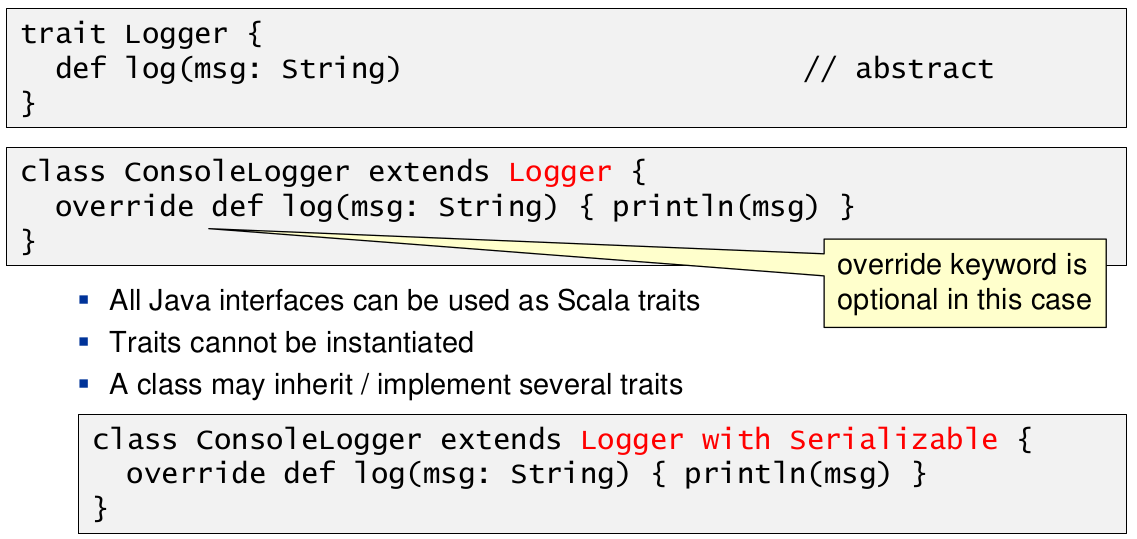
\includegraphics[width=0.7\textwidth]{figures/exampleTrait.png}
\caption{Example Trait}
\end{figure}

The code word \texttt{with} defines a union type. This means, this is a
valid type. If you want to have a combination of two types, you don't
have to create an interface of this two types, you can just use
\texttt{with}.

\begin{lstlisting}[language=scala,mathescape=false]
class ConsoleLogger extends Logger with Serializable with Cloneable {
    override def log(msg: String) { println(msg) }
}
\end{lstlisting}

\hypertarget{trais-with-implementation}{%
\paragraph{Trais with implementation}\label{trais-with-implementation}}

Traits can alos have concrete implementations.

\begin{lstlisting}[language=scala,mathescape=false]
trait ConsoleLogger {
    def log(msg: String) { println(msg) }
}
class DebitAccount extends Account with ConsoleLogger {
    def withdraw(amount: Double) {
        log(s"withdraw($amount) called")
        balance -= amount
    }
    ...
}
\end{lstlisting}

This methods can also be overriden.

\begin{lstlisting}[language=scala,mathescape=false]
trait ConsoleLogger {
    def log(msg: String) { println(msg) }
}
class DebitAccount extends Account with ConsoleLogger {
    def withdraw(amount: Double) {
        log(s"withdraw($amount) called")
        balance -= amount
    }
    override def log(msg: String) {
        super.log("DebitAccount."+msg)
    }
    ...
}
\end{lstlisting}

\hypertarget{traits-on-objects}{%
\paragraph{Traits on objects}\label{traits-on-objects}}

Traits can be added on object at creation time

\begin{lstlisting}[language=scala,mathescape=false]
trait Logger {
    def log(msg: String) { }
}
trait ConsoleLogger extends Logger {
    override def log(msg: String) { println(msg) }
}
class DebitAccount extends Account with Logger {
    def withdraw(amount: Double) {
        log(s"withdraw($amount) called")
        balance -= amount
    }
    ...
}

val a0 = new DebitAccount //Nothing is logged as default logger is used
val a1 = new DebitAccount with ConsoleLogger //On a1, console logger is used for logging
val a2 = new DebitAccount with FileLogger //On a2, a file logger is used
\end{lstlisting}

\hypertarget{extending-interfaces}{%
\subsubsection{Extending Interfaces}\label{extending-interfaces}}

Traits can have utility methods which depend on a few abstract methods
which are provided by the class in which the trait is mixed in. Traits
can also be used to extend the functionality of an interface.

\begin{itemize}
\tightlist
\item
  A class (may be a trait) defines a thin interface which is implemented
  by concrete extensions
\item
  A trait defines additional functionality which may be mixed in
\end{itemize}

\begin{lstlisting}[language=scala,mathescape=false]
trait Logger {
    def log(msg: String) // abstract
    def info(msg: String) { log("INFO: " + msg) }
    def warn(msg: String) { log("WARN: " + msg) }
    def error(msg: String) { log("ERROR: " + msg) }
}
\end{lstlisting}

\clearpage
\hypertarget{stackable-modifications}{%
\subsubsection{Stackable Modifications}\label{stackable-modifications}}

\begin{itemize}
\tightlist
\item
  Traits can be used to modify the behavior, comparable to the decorator
  design pattern
\item
  In contrast to the decorator, traits are mixed in statically and not
  at run-time

  \begin{itemize}
  \tightlist
  \item
    in a class
  \item
    when instances are created
  \end{itemize}
\item
  A particular trait cannot be mixed in several times

  \begin{itemize}
  \tightlist
  \item
    no repeated modifications
  \end{itemize}
\item
  In contrast to the decorator the modified class inherits the types of
  the unmodified class!
\item
  Example

  \begin{itemize}
  \tightlist
  \item
    Timestamp Logger: adds a time stamp
  \item
    Short Logger: shortens the messages
  \end{itemize}
\end{itemize}

\begin{lstlisting}[language=scala,mathescape=false]
//Timestamp Logger
trait TimestampLogger extends Logger {
    override def log(msg: String) {
        super.log(s"${new java.util.Date()} $msg")
    }
}

//Short Logger
trait ShortLogger extends Logger {
    override def log(msg: String) {
        super.log(if(msg.length <= 15) msg else msg.substring(0,12)+"...")
    }
}

scala> val a1 = new DebitAccount with ConsoleLogger with TimestampLogger with ShortLogger
scala> val a2 = new DebitAccount with ConsoleLogger with ShortLogger with TimestampLogger

scala> a1.withdraw(100)
Wed Mai 15 22:38:56 CET 2019 withdraw(100...
scala> a2.withdraw(100)
Wed Mai 15 2...
\end{lstlisting}

\begin{itemize}
\tightlist
\item
  \texttt{super.log} invokes the next trait in the trait hierarchy
\item
  With traits, super calls are dynamically bound, i.e.~you cannot tell
  from the source code of a trait which method is invoked by
  \texttt{super.someMethod}
\end{itemize}

\clearpage
\hypertarget{overriding-abstract-methods-in-traits}{%
\paragraph{Overriding abstract methods in
traits}\label{overriding-abstract-methods-in-traits}}

\begin{itemize}
\tightlist
\item
  If the method in the base trait is abstract, then the overriding
  method in a sub-trait has to be declared both abstract and override
\item
  Abstract override method provides an implementation based on another
  implementation (therefore it is abstract)
\item
  Such an implementation is abstract as it needs a concrete method in a
  class or trait where it can be mixed in
\item
  Supercall still possible but dynamically resolved (invokes provided
  implementation)
\end{itemize}

\begin{lstlisting}[language=scala,mathescape=false]
abstract class IntQueue {
    def get() : Int
    def put(x: Int)
}
class BasicIntQueue extends IntQueue {
    private val buf = new scala.collection.mutable.ArrayBuffer[Int]
    def get() = buf.remove(0) // removes first element
    def put(x: Int) { buf += x } // adds at the end
}

scala> val q = new BasicIntQueue
q: BasicIntQueue = BasicIntQueue@1a6601c
scala> q.put(10); q.put(11);
scala> q.get
res1: Int = 10

//Now with the modificator
trait Doubling extends IntQueue {
    abstract override def put(x: Int) { super.put(2*x); }
}
trait Incr extends IntQueue {
    abstract override def put(x: Int) { super.put(x+1); }
}

//First only with Doubling Queue
scala> val q = new BasicIntQueue with Doubling
q: BasicIntQueue with Doubling = $anon$1@d5714b
scala> q.put(10)
scala> q.get
res32: Int = 20

//Additonal example on multiple traits
scala> val q = new BasicIntQueue with Doubling with Incr
q: BasicIntQueue with Doubling with Incr = $anon$1@3b60efd8
scala> q.put(10)
scala> q.get //22
scala> val q = new BasicIntQueue with Incr with Doubling
q: BasicIntQueue with Incr with Doubling = $anon$1@61598d13
scala> q.put(10) 
scala> q.get //21
\end{lstlisting}

\clearpage
\hypertarget{self-types}{%
\subsubsection{Self Types}\label{self-types}}

\begin{itemize}
\tightlist
\item
  If a trait extends a class C, that class becomes a superclass of any
  class mixing in the trait
\item
  Alternatively one can define the self type to guarantee that the trait
  is mixed in a particular class
\item
  In the trait methods, any methods of the self type can be invoked
\end{itemize}

\begin{lstlisting}[language=scala,mathescape=false]
//Name of the self type is irrelevant, could be named self (or ex or ...)
trait ExceptionLogger extends Logger {
    this: Exception =>
    def log() { log(getMessage()) }
}
\end{lstlisting}

\hypertarget{class-linearization}{%
\subsection{Class Linearization}\label{class-linearization}}

\textit{Leading question: In which order are the traits called?}

When an instance of a class C is created with new C, then the class C
and all its inherited classes and traits are put in a \textbf{single,
linear order}.

\begin{itemize}
\tightlist
\item
  The linear order defines the constructor invocation order (from Any to
  C)
\item
  The linear order defines method lookup priorities, i.e.~it defines,
  which method overrides another method
\item
  The linear order defines which method is called on a super call (it is
  the next in the linear order chain)
\end{itemize}

\textbf{No diamond problems and each class appears only once!}

\begin{itemize}
\tightlist
\item
  The inheritance relationship on base classes forms in general a DAG
\item
  A linearization of this graph is defined as follows:
\end{itemize}

\begin{figure}[H]
\centering
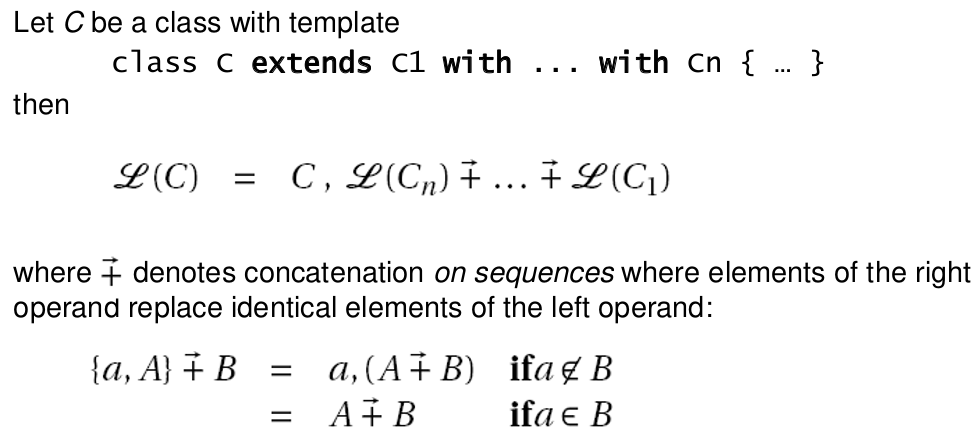
\includegraphics[width=0.5\textwidth]{figures/classLinearization.png}
\caption{Class Linearization}
\end{figure}

\begin{enumerate}
\def\labelenumi{\arabic{enumi}.}
\tightlist
\item
  Put the actual type of the instance as the first element
\item
  Starting with the rightmost parent type and working from right to
  left, compute the linearization of each type, appending its
  linearization to the cumulative linearization
\item
  Working from left to right, remove any type if it appears again to the
  right of the current position
\item
  Append AnyRef and Any
\end{enumerate}

\hypertarget{example}{%
\subsubsection{Example}\label{example}}

\begin{figure}[H]
\centering
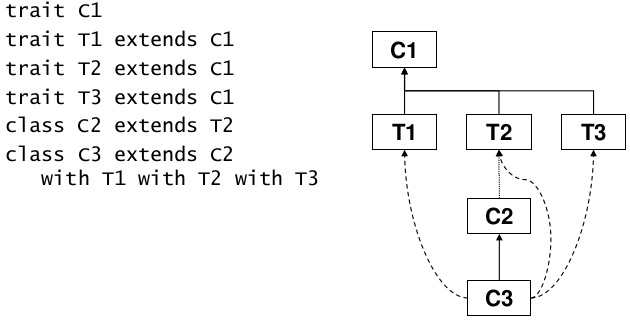
\includegraphics[width=0.5\textwidth]{figures/classLinearizationExample.png}
\caption{Class Linearization Example}
\end{figure}

\begin{figure}[H]
\centering
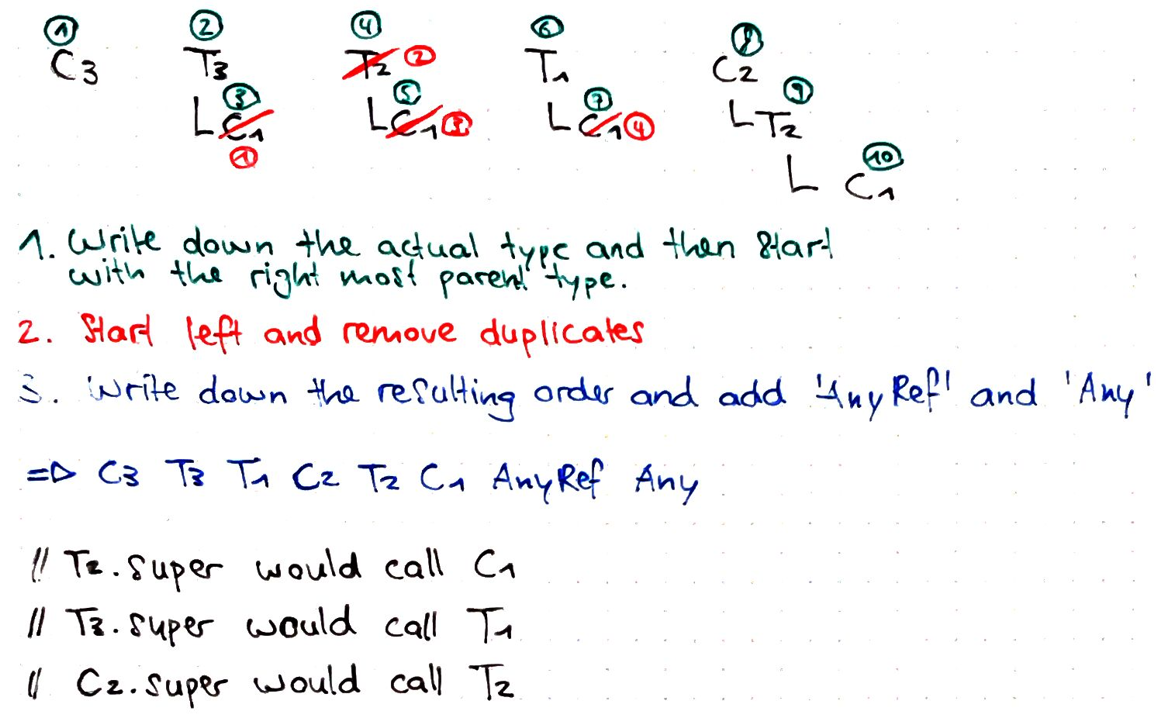
\includegraphics[width=0.7\textwidth]{figures/classLinearization2.png}
\caption{Class Linearization Example}
\end{figure}

\hypertarget{super-call-to-specific-class}{%
\subsubsection{Super Call to specific
class}\label{super-call-to-specific-class}}

\begin{itemize}
\tightlist
\item
  Scala allows to qualify the super call
\item
  Qualification can't refer to a grandparent type, only directly
  inherited classes and traits (in the direction of right)
\end{itemize}

\begin{lstlisting}[language=scala,mathescape=false]
super[T2].print
\end{lstlisting}

\clearpage
\hypertarget{applications}{%
\subsection{Applications}\label{applications}}

\begin{itemize}
\tightlist
\item
  Interfaces

  \begin{itemize}
  \tightlist
  \item
    Traits are used to mimic Java interfaces
  \end{itemize}
\item
  Abstract Classes

  \begin{itemize}
  \tightlist
  \item
    Traits are used to mimic abstract classes known in Java (or Java-
    Interfaces with default methods)
  \end{itemize}
\item
  Widening thin interfaces to rich ones

  \begin{itemize}
  \tightlist
  \item
    Default methods are added in a trait and can be mixed in a class
    which implements the abstract (thin) layer
  \end{itemize}
\item
  Defining stackable modifications

  \begin{itemize}
  \tightlist
  \item
    Several traits extending (or restricting themselves) to a common
    base class are stacked (or chained) in different orders to modify
    the behavior
  \item
    Decorator pattern

    \begin{itemize}
    \tightlist
    \item
      But traits can only be applied statically at compile time
    \item
      On the other hand type of decorated object is preserved
    \end{itemize}
  \end{itemize}
\end{itemize}

\hypertarget{compound-types}{%
\subsubsection{Compound Types}\label{compound-types}}

If I have two different traits or types, I can combine them using
\texttt{with}. These types are union types and define a new type. The
combined types don't need to know each other.

\clearpage
\hypertarget{scala-types}{%
\section{Scala - Types}\label{scala-types}}

\begin{figure}[H]
\centering
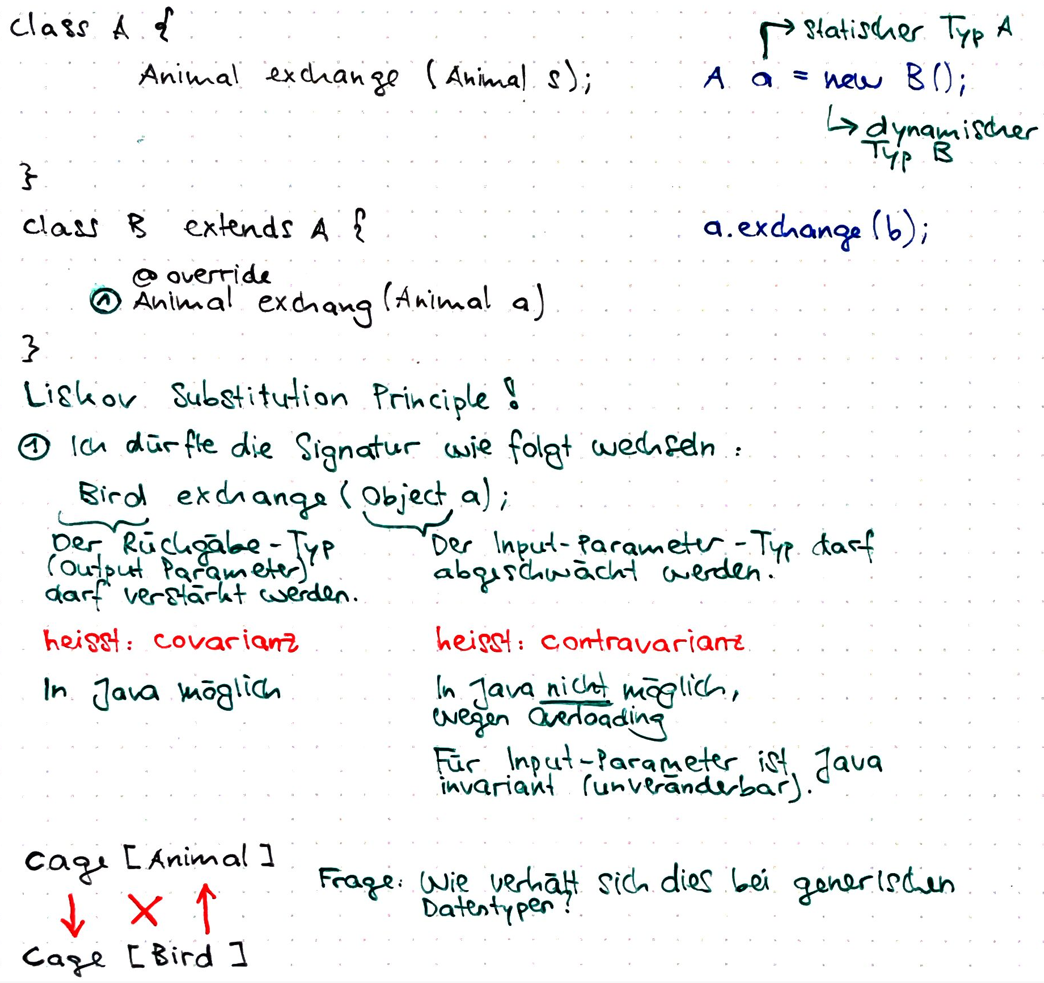
\includegraphics[width=0.85\textwidth]{figures/scalaVarianceIntro.png}
\caption{Variance Introduction}
\end{figure}

\hypertarget{parameterized-types}{%
\subsection{Parameterized Types}\label{parameterized-types}}

\hypertarget{generic-classes}{%
\subsubsection{Generic Classes}\label{generic-classes}}

\begin{lstlisting}[language=scala,mathescape=false]
case class Pair[T, S](val first: T, val second: S)

scala> val p1 = Pair(42, "String")
p1: Pair[Int,String] = Pair@4c5853eb
\end{lstlisting}

\hypertarget{generic-functions}{%
\subsubsection{Generic Functions}\label{generic-functions}}

\begin{lstlisting}[language=scala,mathescape=false]
def getMiddle[T](a: Array[T]) = a(a.length / 2)

scala> getMiddle(Array("one", "two", "three"))
res1: String = two
scala> getMiddle(Array(1, "two"))
res2: Any = two
\end{lstlisting}

\hypertarget{type-variable-bounds}{%
\subsubsection{Type Variable Bounds}\label{type-variable-bounds}}

\textbf{Upper Bounds}

\begin{lstlisting}[language=scala,mathescape=false]
case class Pair[T <: Comparable[T]](val p1: T, val p2: T) {
    def smaller = if(p1.compareTo(p2) < 0) p1 else p2
}

scala> val p = Pair("Stan", "Ollie")
p: Pair[String] = Pair(Stan,Ollie)
scala> p.smaller
res10: String = Ollie
scala> Pair(List("one"), List("two"))
error: inferred type arguments [List[String]] do not conform to class Pair's type parameter bounds [T <: Comparable[T]] new Pair(List("one"), List("two"))
\end{lstlisting}

This throws an error, since Lists do not implement Comparable.

\textbf{Lower Bounds}

\begin{lstlisting}[language=scala,mathescape=false]
case class Pair[T](val p1: T, val p2: T) {
    def setFirst(newP1: T) = new Pair[T](newP1, p2)
}

scala> val p = Pair("one", "two")
p: Pair[String] = Pair(one,two)
scala> p.setFirst(1)
<console>:13: error: type mismatch;
found    : Int(1)
required : String
            p.setFirst(1)
\end{lstlisting}

Since Pair is immutable, a new instance has to be created. With the
above definition, the resulting pair (when calling setFirst) is always
of the same type, even if something more general is added.

\begin{lstlisting}[language=scala,mathescape=false]
case class Pair[T](val p1: T, val p2: T) {
    def setFirst[R >: T](newP1: R) = new Pair[R](newP1, p2)
}

scala> val p = Pair("one", "two")
p: Pair[String] = Pair(one,two)
scala> p.setFirst(1)
res1: Pair[Any] = Pair(1,two)
scala> p.setFirst(null)
res2: Pair[String] = Pair(null,two)
\end{lstlisting}

The replacement type for the type variable of the new pair must be a
supertype of the pair's component type T

\hypertarget{bounds}{%
\subsubsection{Bounds}\label{bounds}}

Multiple lower and upper bounds can be specified with a compound type

\begin{lstlisting}[language=scala,mathescape=false]
def foo[T <: Comparable[T] with Serializable](x: T) = x
\end{lstlisting}

A type variable can have both an upper and a lower bound

\begin{lstlisting}[language=scala,mathescape=false]
// T >: Lower <: Upper
scala> class MBounds[T >: String <: AnyRef]
scala> new MBounds[String]
res1: MBounds[String] = MBounds@5fc59667
scala> new MBounds[CharSequence]
res2: MBounds[CharSequence] = MBounds@794579f3
scala> new MBounds[AnyRef]
res3: MBounds[AnyRef] = MBounds@4f028abf
\end{lstlisting}

\hypertarget{variance}{%
\subsection{Variance}\label{variance}}

It depends on the situation, which variance should apply or not.

\begin{figure}[H]
\centering
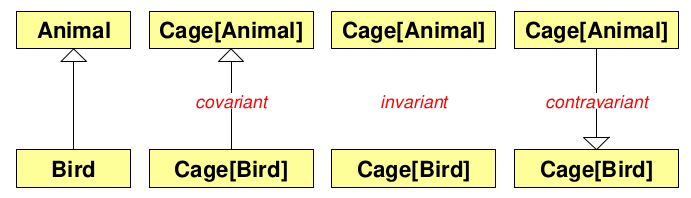
\includegraphics[width=0.7\textwidth]{figures/coAndContravarianz.png}
\caption{Variance}
\end{figure}

\begin{itemize}
\tightlist
\item
  If I only read from the object I receive, then the object need to be
  covariant (like output parameter)
\item
  If I only write to the object I receive, then the object need to be
  contravariant (like input parameter)
\item
  If I read and write from and to the object, the object needs to be
  invariant
\end{itemize}

\hypertarget{variance-in-java}{%
\subsubsection{Variance in Java}\label{variance-in-java}}

In Java, generic types are basically invariant, but you are able to
specify covariance or contravariance with super or extends.

Generics:

\begin{lstlisting}[language=scala,mathescape=false]
public class Test1 {
    static class Animal {}
    static class Bird extends Animal {}
    static class Cage<T> {}
    public static void main(String[] args) {
        Cage<Bird> birdCage = new Cage<Bird>();
        Cage<Animal> animalCage;
        animalCage = birdCage;
    }
}

//Compiler Error: Type mismatch:
//cannot convert from Cage<Bird> to Cage<Animal>
\end{lstlisting}

Arrays:

\begin{lstlisting}[language=scala,mathescape=false]
public class Test2 {
    static class Animal {}
    static class Bird extends Animal {}
    public static void main(String[] args) {
        Bird[] birdCage = new Bird[1];
        Animal[] animalCage = birdCage;
        animalCage[0] = new Animal();
    }
}

//Runtime Error: Exception in thread "main"
//java.lang.ArrayStoreException: Test2$Animal
//at Test2.main(Test2.java:12)
\end{lstlisting}

Wird auf ein Element im Array zugegriffen, wird jedes mal geprüft ob es
sich beim aktuellen Element um den dynamischen Typ des Arrays handelt
(und nicht um den statischen Typs).

\hypertarget{variance-in-scala}{%
\subsubsection{Variance in Scala}\label{variance-in-scala}}

\textbf{\textit{Read-only (immutable) =\textgreater{} covariant}}\\
A bird cage can be considered as a special animal cage (as it also
contains an animal =\textgreater{} expectation met!)

\textbf{\textit{Write-only =\textgreater{} contravariant}}\\
An animal cage can be considered a special bird cage (as it can be used
to put birds in it =\textgreater{} expectation met!)

\begin{lstlisting}[language=scala,mathescape=false]
scala> class Animal; class Bird extends Animal
scala> class Cage[A]
scala> val animalCage: Cage[Animal] = new Cage[Bird]
<console>:14: error: type mismatch;
found: Cage[Bird]
required: Cage[Animal]
Note: Bird <: Animal, but class Cage is invariant in type A.
You may wish to define A as +A instead. (SLS 4.5)

scala> val birdCage: Cage[Bird] = new Cage[Animal]
<console>:14: error: type mismatch;
found: Cage[Animal]
required: Cage[Bird]
Note: Animal >: Bird, but class Cage is invariant in type A.
You may wish to define A as -A instead. (SLS 4.5)
\end{lstlisting}

\textbf{Covariance} 

Use + to declare a covariant type parameter

\begin{lstlisting}[language=scala,mathescape=false]
scala> class Animal; class Bird extends Animal
scala> class Cage[+A]

scala> val animalCage: Cage[Animal] = new Cage[Bird]
animalCage: Cage[Animal] = Cage@62d75a88

scala> val birdCage: Cage[Bird] = new Cage[Animal]
<console>:14: error: type mismatch;
\end{lstlisting}

\textbf{Contravariant}

Use - to declare a contravariant type parameter

\begin{lstlisting}[language=scala,mathescape=false]
scala> class Animal; class Bird extends Animal
scala> class Cage[-A]

scala> val animalCage: Cage[Animal] = new Cage[Bird]
<console>:14: error: type mismatch;

scala> val birdCage: Cage[Bird] = new Cage[Animal]
birdCage: Cage[Bird] = Cage@1bdab192
\end{lstlisting}

\textbf{Drawbacks}

When can we use variance declarations on class type params?\\
The answer depends on whether type variables are used in producer
(positive) or consumer (negative) positions

\begin{itemize}
\tightlist
\item
  To be safe for covariance, a type parameter T must appear only in
  ``producer'' (positive) positions in method signatures
\item
  To be safe for contravariance, a type parameter T must appear only in
  ``consumer'' (negative) positions in method signatures
\end{itemize}

\begin{lstlisting}[language=scala,mathescape=false]
abstract class Cage [A] {
    def get: A              //+
    def put(a: A): Unit     //-
    val animal: A           //+ (because immutable)
    var animal2: A          //+-
}
\end{lstlisting}

The Scala compilers throws an error if these rules are harmed.

\textbf{Variance Declarations and Subclassing}

\begin{lstlisting}[language=scala,mathescape=false]
class Cage[A] // invariant
class SpecialCage[+A] extends Cage[A] // not ok
class SpecialCage[ A] extends Cage[A] // ok
class SpecialCage[-A] extends Cage[A] // not ok

class Cage[+A] // covariant
class SpecialCage[+A] extends Cage[A] // ok
class SpecialCage[ A] extends Cage[A] // ok
class SpecialCage[-A] extends Cage[A] // not ok

class Cage[-A] // contravariant
class SpecialCage[+A] extends Cage[A] // not ok
class SpecialCage[ A] extends Cage[A] // ok
class SpecialCage[-A] extends Cage[A] // ok
\end{lstlisting}

\hypertarget{variance-in-java-bounded-wildcards}{%
\subsubsection{Variance in Java: Bounded
Wildcards}\label{variance-in-java-bounded-wildcards}}

Java controls variance on use-site (not on declaration site)

\begin{lstlisting}[language=scala,mathescape=false]
//Covariance
void readAnimal(Cage<? extends Animal> cage) {
    Animal a = cage.getContent();
}
//One can only read from the cage

//Contravariance
void storeBird(Bird b, Cage<? super Bird> cage) {
    cage.setContent(b);
}
//One can't read anymore. 
//On the parameter cage, only methods can be invoked which have the type parameter in a contravariant position
\end{lstlisting}

\clearpage
\textbf{Example}

\begin{lstlisting}[language=scala,mathescape=false]
class A {}
class B extends A {}
class C extends B {}
class Cage<T extends A> {
    private T x;
    public T getContent() { return x; }
    public void setContent(T a) { x = a; }
    public T replaceContent(T a) { T ret = x; x = a; return ret; }
}

public static void readContent(Cage<? extends B> cage) {
    B b = cage.getContent();
    // cage.setContent(new B()); // method not applicable
    // a = cage.replaceContent(new B());
    cage.setContent(null);
    b = cage.replaceContent(null);
}

public static void writeContent(Cage<? super B> cage) {
    // B b = cage.getContent();
    // type mismatch
    cage.setContent(new B());
    // b = cage.replaceContent(new B()); // type mismatch
}
\end{lstlisting}

\hypertarget{problems}{%
\paragraph{Problems}\label{problems}}

\begin{itemize}
\tightlist
\item
  Types on use-site can get complicated, with nesting of variance
  annotations
\item
  Annotations must be maintained on every use of a generic type
\end{itemize}

\hypertarget{comments}{%
\paragraph{Comments}\label{comments}}

\begin{itemize}
\tightlist
\item
  Declaration-site variance is the choice if the language prefers
  immutable data structures
\item
  Use-site variance is just right for mutable (invariant) data
  structures. It gives each service the choice which variance, if any,
  is appropriate
\end{itemize}

\clearpage
\hypertarget{scala-types}{%
\section{Scala - More Types}\label{scala-types}}

\hypertarget{inner-types}{%
\subsection{Inner Types}\label{inner-types}}

Classes, traits and singleton objects can have inner types, i.e.

\begin{itemize}
\tightlist
\item
  Inner classes
\item
  Inner traits
\item
  Inner type members
\end{itemize}

\begin{lstlisting}[language=scala,mathescape=false]
class Outer {
    class InnerClass
    trait InnerTrait
    type InnerType = String
}
\end{lstlisting}

\hypertarget{path-dependent-types}{%
\subsubsection{Path-dependent Types}\label{path-dependent-types}}

To access an inner type you need an outer instance

\begin{lstlisting}[language=scala,mathescape=false]
class Outer {
    class Inner
    def put(inner: /* optional: this.*/Inner) {}
}
defined class Outer

scala> val outer1 = new Outer
outer1: Outer = Outer@6ef8fff2

scala> val inner1 = new outer1.Inner
inner1: outer1.Inner = Outer$Inner@11c7d2e3
\end{lstlisting}

The type of an inner instance depends on the outer instance

\begin{lstlisting}[language=scala,mathescape=false]
scala> val outer2 = new Outer
outer2: Outer = Outer@73a1deca

scala> val inner2 = new outer2.Inner
inner2: outer2.Inner = Outer$Inner@1a1dd898

scala> outer1.put(inner2)
<console>:14: error: type mismatch;
found   : outer2.Inner
required: outer1.Inner
\end{lstlisting}

The inner types share a common supertype, denoted by a type selection
Outer\#Inner

\begin{lstlisting}[language=scala,mathescape=false]
class Outer {
    class Inner
    def put(inner: Outer#Inner) {}
}
defined class Outer

scala> val inner1: Outer#Inner = new outer1.Inner
inner1: Outer#Inner = Outer$Inner@502c500d

scala> val inner2: Outer#Inner = new outer2.Inner
inner2: Outer#Inner = Outer$Inner@7e912427

scala> outer2.put(inner1)
\end{lstlisting}

\hypertarget{dependent-types}{%
\subsubsection{Dependent Types}\label{dependent-types}}

Dependent types are types which depend on a value. They can be emulated
with path dependent types.

\begin{lstlisting}[language=scala,mathescape=false]
object Arrays {
    case class OfLength(n: Int) {
        class Arr {
            private val a: Array[Int] = new Array[Int](n)
            def apply(x: Int) = a(x)
            def update(x: Int, y: Int): Unit = {a(x) = y}
        }
    }
    // The following types are two different types
    val ofLength4 = OfLength(4)
    val ofLength5 = OfLength(5)

    type ArrayOfLength4 = ofLength4.Arr
    type ArrayOfLength5 = ofLength5.Arr

    def f(a: ArrayOfLength5): Unit = { a(4) = 4 }

    val a4 = new ArrayOfLength4
    val a5 = new ArrayOfLength5

    f(a5) // <<= OK
    f(a4) // <<= type error
    //<console> :14: error: type mismatch;
    //found     : ofLength4.Arr
    //required  : ArrayOfLength5
    //(which expands to) ofLength5.Arr
}
\end{lstlisting}

\hypertarget{singleton}{%
\subsection{Singleton}\label{singleton}}

Singleton type is a type which represents a reference. Given any
reference v, the type v.type has two values: v and null.

\begin{lstlisting}[language=scala,mathescape=false]
scala> class X
defined class X
scala> val x = new X
x: X = X@12d05dde
scala> var y: x.type = x
y: x.type = X@12d05dde
scala> y = null
y: x.type = null
scala> y = new X
<console>   :13: error: type mismatch;
found       : X
required    : x.type
\end{lstlisting}

\clearpage
\hypertarget{application-1-method-chaining-fluent-interfaces}{%
\subsubsection{Application 1: Method Chaining (fluent
interfaces)}\label{application-1-method-chaining-fluent-interfaces}}

Fluent interface is a method for designing object oriented APIs based
extensively on method chaining with the goal of making the readability
of the source code close to that of ordinary written prose.

\begin{lstlisting}[language=scala,mathescape=false]
class Document {
    def setTitle(title: String) = { ...; this }
    def setAuthor(author: String) = { ...; this }
    ...
}

article.setAuthor("Horstmann").setTitle("Scala")

class Book extends Document {
    def addChapter(chapter: String) = { ...; this }
    ...
}

val book = new Book()
book.setTitle("Scala").addChapter(chapter1)
error: value addChapter is not a member of Document
\end{lstlisting}

With an additional statement, one can preserve the original type in the
class:

\begin{lstlisting}[language=scala,mathescape=false]
class Document {
    def setTitle(title: String): this.type = { ...; this }
    def setAuthor(author: String): this.type = { ...; this }
    ...
}
class Book extends Document {
    def addChapter(chapter: String) = { ...; this }
    ...
}

scala> book.setTitle("Scala").addChapter("ch1")
res32: Book = Book@5213fe32
scala> book.setTitle("Scala")
res33: book.type = Book@5213fe3
\end{lstlisting}

\hypertarget{application-2-fluent-interfaces}{%
\subsubsection{Application 2: Fluent
interfaces}\label{application-2-fluent-interfaces}}

\begin{lstlisting}[language=scala,mathescape=false]
object Title
class Document {
    var title: String = ""
    private var useNextArgAs: Any = null
    def set(obj: Title.type) = { useNextArgAs = obj; this }
    def to(arg: String) = {
        if(useNextArgAs == Title) { title = arg; } // else ...
    }
    //...
}
val book = new Document
book.set(Title).to("Scala")

book set Title to "Scala"
//In scala it is possible to leave away the paranthesis and the dots, if there is only one parameter.
\end{lstlisting}

\clearpage
\hypertarget{implicits}{%
\subsection{Implicits}\label{implicits}}

\hypertarget{implicit-conversions}{%
\subsubsection{Implicit Conversions}\label{implicit-conversions}}

Implicit conversion function

\begin{itemize}
\tightlist
\item
  Method or function with one argument (method name is irrelevant)
\item
  Marked with the implicit keyword
\item
  The compiler knows how to compile the given type to the target type

  \begin{itemize}
  \tightlist
  \item
    e.g.~when actually a Fraction is required but the given type is
    integer, the compiler realizes that there is a converter.
  \end{itemize}
\end{itemize}

\begin{lstlisting}[language=scala,mathescape=false]
import scala.language.implicitConversions
implicit def int2Fraction(n: Int) = Fraction(n,1)

scala> val f1: Fraction = 2
f1: Fraction = Fraction(2,1)
scala> 3 * Fraction(4,5)
res2: Fraction = Fraction(12,5)
\end{lstlisting}

Another example

\begin{lstlisting}[language=scala,mathescape=false]
//Could also write "implicit class BlingString(string: String) {.." and leave the "implicit def ..." away.

class BlingString(string: String) {
    def bling = "*" + string + "*"
}
implicit def blingToString(s: String) = new BlingString(s)

scala> "Hello".bling
res1: String = *Hello*

scala> "Hello".bling.bling
res2: String = **Hello**
\end{lstlisting}

Instead of creating a new instance for every application, a value class
can be used

\begin{itemize}
\tightlist
\item
  Value classes avoid creation of objects
\item
  Value class has a single public val parameter that is the underlying
  runtime representation
\item
  Has only defs as members, but no vals, vars, or nested traits, classes
  or objects
\end{itemize}

\begin{lstlisting}[language=scala,mathescape=false]
implicit class BlingString(val string: String) extends AnyVal {
    def bling = "*" + string + "*"
}
\end{lstlisting}

\hypertarget{implicit-conversion-rules}{%
\subsubsection{Implicit Conversion
Rules}\label{implicit-conversion-rules}}

Implicit conversions are considered in three cases.

If the type of an expression differs from the expected type

\begin{lstlisting}[language=scala,mathescape=false]
val f: Fraction = 12
\end{lstlisting}

If a non-existent member is accessed

\begin{lstlisting}[language=scala,mathescape=false]
"hello".bling
\end{lstlisting}

If an object invokes a method whose parameters don't match the given
arguments

\begin{lstlisting}[language=scala,mathescape=false]
3 * Fraction(4,5) // Int.* does not accept a Fraction arg
\end{lstlisting}

In order to be applied, an implicit conversion must be in scope

Current scope: Identifiers accessible without prefix

\begin{itemize}
\tightlist
\item
  Local identifiers

  \begin{itemize}
  \tightlist
  \item
    Members of an enclosing scope
  \item
    Imported identifiers
  \end{itemize}
\item
  Implicit scope: Members of companion objects of associated types

  \begin{itemize}
  \tightlist
  \item
    The types in question (source or target type)
  \item
    All parts of a parameterized type, e.g.~A{[}B,C{]}
  \item
    All parts of a compound type, e.g.~A with B with C
  \end{itemize}
\item
  Precedence rules

  \begin{itemize}
  \tightlist
  \item
    Local implicits
  \item
    Imported implicits
  \item
    Companion object of the types
  \item
    Companion object of the type arguments of the type
  \end{itemize}
\end{itemize}

\hypertarget{implicit-parameters}{%
\subsubsection{Implicit Parameters}\label{implicit-parameters}}

\begin{itemize}
\tightlist
\item
  Use the keyword implicit to define an implicit parameter list
\item
  This only works for the last parameter list
\end{itemize}

\begin{lstlisting}[language=scala,mathescape=false]
case class Delimiters(left: String, right: String)

def quote(text: String)(implicit delims: Delimiters) = delims.left + text + delims.right

scala> quote("Bonjour")(Delimiters("<<", ">>")) // Guillemets
res1: String = <<Bonjour>>

scala> quote("Hello")
<console>:14: error: could not find implicit value for parameter
delims: Delimiters
\end{lstlisting}

For this, one can define which implicit types should be used, if nothing
is given with the function.

\begin{lstlisting}[language=scala,mathescape=false]
import java.io.PrintStream
import java.lang._
implicit val out = System.out

def log(msg: String)(implicit out: PrintStream) = out.println(msg)

scala> log("Implicits are cool")
Implicits are cool

scala> log("here is an error")(System.err)
here is an error
\end{lstlisting}

\hypertarget{type-classes}{%
\subsection{Type classes}\label{type-classes}}

Type classes are among the most powerful features in Haskell. They allow
you to define generic interfaces that provide a common feature set over
a wide variety of types. Type classes are at the heart of some basic
language features such as equality testing and numeric operators.

\begin{itemize}
\tightlist
\item
  Type classes define a group (class) of types which satisfy some
  contract (defined in a trait)
\item
  Type classes add ad-hoc polymorphism
\item
  Example: sort method on a list
\end{itemize}

\begin{lstlisting}[language=scala,mathescape=false]
scala> List(3,2,1).sorted
res12: List[Int] = List(1, 2, 3)
\end{lstlisting}

What constraint is defined on the type parameter?

\begin{itemize}
\tightlist
\item
  class List{[}A \textless{}: Comparable{[}A{]}{]} \{ \ldots{} \}
\item
  def sorted\href{implicit\%20ord:\%20math.Ordering\%5BB\%5D}{B
  \textgreater{}: A}: List{[}A{]}
\end{itemize}

\hypertarget{polymorphism}{%
\subsubsection{Polymorphism}\label{polymorphism}}

\begin{itemize}
\tightlist
\item
  Ad-hoc polymorphism

  \begin{itemize}
  \tightlist
  \item
    Different implementations depending on the parameter types
  \item
    Method overloading is one example of ad-hoc polymorphism
  \end{itemize}
\item
  Parametric polymorphism

  \begin{itemize}
  \tightlist
  \item
    Code to be used transparently with any number of new types
  \item
    Generics is an example of parametric polymorphism
  \end{itemize}
\item
  Subtype polymorphism
\item
  Subtyping allows a function to be written to take an object of a
  certain type T, but also work correctly with subtypes of T
  (=\textgreater{} Liskov substitution principle)
\end{itemize}

\hypertarget{monoid}{%
\subsubsection{Monoid}\label{monoid}}

\begin{lstlisting}[language=scala,mathescape=false]
trait Monoid[A] {
    def op(x: A, y: A) : A
    def unit : A
}

//Two implementations
implicit object stringMonoid extends Monoid[String] {
    def op(x: String, y: String) = x + y
    def unit = ""
}
implicit object addMonoid extends Monoid[Int] {
    def op(x: Int, y: Int) = x + y
    def unit = 0
}

//Object of Monoid
object Monoid {
    def apply[A](implicit m: Monoid[A]) = m
}

scala> Monoid[String]
res1: Monoid[String] = stringMonoid$@64fc6470
scala> Monoid[Int]
res2: Monoid[Int] = addMonoid$@680937c9
\end{lstlisting}

\hypertarget{use-monoids-for-a-list-accumulator}{%
\subsubsection{Use Monoids for a List
accumulator}\label{use-monoids-for-a-list-accumulator}}

\begin{lstlisting}[language=scala,mathescape=false]
def acc[A](list: List[A])(implicit m: Monoid[A]) : A = list.foldLeft(m.unit)(m.op)

scala> acc(List(1,2,3))
res1: Int = 6

scala> acc(List("Hello", "World"))
res2: String = HelloWorld

scala> acc(List(List(1), List(1,2), List(1,2,3)))
<console>:12: error: could not find implicit value for parameter m:
Monoid[List[Int]]
\end{lstlisting}

\hypertarget{conditional-implicits}{%
\subsubsection{Conditional implicits}\label{conditional-implicits}}

Implicit methods can themselves have implicit parameters. This is super
fancy!

\begin{lstlisting}[language=scala,mathescape=false]
implicit def listMonoid[A](implicit m: Monoid[A]) =
    new Monoid[List[A]] {
        def op(xs: List[A], ys: List[A]): List[A] =
            if(xs.isEmpty) ys
            else if (ys.isEmpty) xs
            else m.op(xs.head, ys.head) :: op(xs.tail, ys.tail)
        def unit = List()
    }
}

scala> acc(List(List(1), List(1,2), List(1,2,3)))
res3: List[Int] = List(3, 4, 3)
//The lists are added element-wise
//[1+1+1, 0+2+2, 0+0+3] = [3, 4, 3]
\end{lstlisting}

\clearpage
\hypertarget{shorthand-notation-for-implicit-parameters}{%
\subsubsection{Shorthand notation for implicit
parameters}\label{shorthand-notation-for-implicit-parameters}}

\begin{lstlisting}[language=scala,mathescape=false]
def acc[A](list: List[A])(implicit m: Monoid[A]) : A = list.foldLeft(m.unit)(m.op)

def acc[A : Monoid](list : List[A]) : A = {
    val m = Monoid[A]
    list.foldLeft(m.unit)(m.op)
}
\end{lstlisting}

\hypertarget{conclusion-to-type-classes}{%
\subsubsection{Conclusion to type
classes}\label{conclusion-to-type-classes}}

Type classes allow us to

\begin{itemize}
\tightlist
\item
  introduce polymorphic functions, extensible (by composition) after the
  original code has been written (by providing new implementations)

  \begin{itemize}
  \tightlist
  \item
    Example: Monoid for String, Int and List{[}A{]}
  \end{itemize}
\item
  introduce generic functions in terms of the prototypes assumed to
  exist

  \begin{itemize}
  \tightlist
  \item
    Example: Method acc
  \end{itemize}
\item
  Implicit resolution

  \begin{itemize}
  \tightlist
  \item
    Implicits are looked for in the local scope (contrary to Haskell)

    \begin{itemize}
    \tightlist
    \item
      Several different implementations can be provided for a particular
      type
    \item
      With imports the implicits to be used are controllable
    \end{itemize}
  \end{itemize}
\end{itemize}

\clearpage
\hypertarget{limitations}{%
\subsubsection{Limitations}\label{limitations}}

The following code shows three classes. Two B classes are derivated from
A and override their own show method.

\begin{lstlisting}[language=scala,mathescape=false]
trait Show { def show: String }
class A extends Show { override def show = "A" }
class B1 extends A { override def show = "B1" }
class B2 extends A { override def show = "B2" }

scala> val list = List(new A, new B1, new B2)
list: List[A] = List(A@16d48c9, B1@2dc584da, B2@2951bb0)
scala> list.map( x => x.show )
res1: List[String] = List(A, B1, B2)
\end{lstlisting}

This can also be done with type classes:

\begin{lstlisting}[language=scala,mathescape=false]
trait Showable[T] { def show(x: T): String }
object Showable {
    implicit object a extends Showable[A]{ def show(x: A) = "TC:A" }
    implicit object b1 extends Showable[B1]{ def show(x: B1) = "TC:B1"}
    implicit object b2 extends Showable[B2] { def show(x: B2) = "TC:B2" }
}
def show[T : Showable](x: T) = {
    implicitly[Showable[T]].show(x)
}
scala> list.map( x => show(x))
res2: List[String] = List(TC:A, TC:A, TC:A)
\end{lstlisting}

As you see, it prints everytime A. This is because the type is evaluated
at compile time and the type of the List is A.

\clearpage
\section{Exercises}

\hypertarget{haskell-types}{%
\subsection{Haskell Types}\label{haskell-types}}

\hypertarget{types-of-lists-and-tuples}{%
\subsubsection{Types of Lists and Tuples}\label{types-of-lists-and-tuples}}

After declare x = `x':

\begin{lstlisting}[language=Haskell]
x ==> Char
'x' ==> Char
"x" ==> [Char]
['x'] ==> [Char]
[x, 'x'] ==> [Char]
[x, x, x, x] ==> [Char]
['x', "x"] ==> error
[x, True] ==> error
[x == 'x', True] ==> [Bool]
[["True"]] ==> [[[Char]]]
[[ True, False], True] ==> error
[[ True, False], []] ==> [[Bool]]
('x') ==> Char
(x , 'x') ==> (Char, Char)
(x ,x, x, x) ==> (Char, Char, Char, Char)
('x', "x") ==> (Char, [Char])
(x , True) ==> (Char, Bool)
(x == 'x' ,True) ==> (Bool, Bool)
(("True")) ==> [Char]
((True ,False) ,True) ==> ((Bool, Bool), Bool)
((True, False), ()) ==> ((Bool, Bool), ())
\end{lstlisting}

\hypertarget{types-of-lists}{%
\subsubsection{Types of Lists}\label{types-of-lists}}

\begin{lstlisting}[language=Haskell]
After declare a = [True]:

a ==> [Bool]
a ++ a ++ [True] ==> [Bool]
a ++ [] ==> [Bool]
head a ==> Bool
tail a (*) ==> error
head 'x' ==> error
head "x" ==> Char
tail "x" (*) ==> error
"dimdi" !! 2 ==> Char (Gibt den dritten Buchstaben aus (0 indexiert))
"dimdi" ++ "ding" ==> [Char]
\end{lstlisting}

\hypertarget{types-of-functions-and-lists}{%
\subsubsection{Types of Functions and
Lists}\label{types-of-functions-and-lists}}

\begin{lstlisting}[language=Haskell]
f1 :: Int -> Int
f1 x = x^2 + x + 1
f2 :: Int -> Int
f2 x = 2 * x + 1

f1 ==> Int -> Int
f1 5 ==> Int
f1 f2 ==> error
f1 (f2 5) ==> Int
[f1 5, f2 6, 5, 6] ==> [Int]
[f1, f2, f1] ==> [Int -> Int]
[f1 5, f2] ==> error
(f1 5, f2) ==> (Int, Int -> Int)
([f1, f2, f1] !! 1) 3 ==> Int
([f1, f2, f1] !! 5) 3 (*) ==> error
\end{lstlisting}

\hypertarget{types-of-functions-with-currying}{%
\subsubsection{Types of Functions with
Currying}\label{types-of-functions-with-currying}}

\begin{lstlisting}[language=Haskell]
g1 :: Int -> Int -> Int -> Int
g1 x y z = x^2 + y^2 + z^2
g2 :: Int -> Int -> Int
g2 x y = 2*x + 2*y

g1  ==> Int -> Int -> Int -> Int
g1 2 ==> Int -> Int -> Int
g1 2 3 ==> Int -> Int
g1 2 3 4 ==> Int
g1 2 3 4 5 ==> eroor
(g1, g2) ==> (Int -> Int -> Int -> Int, Int -> Int -> Int)
(g1 2, g2) ==> (Int -> Int -> Int, Int -> Int -> Int)
(g1 2 3, g2 4) ==> (Int -> Int, Int -> Int)
(g1 2 3 4, g2 4 5) ==> (Int, Int)
[g1, g2] ==> error
[g1 2, g2] ==> [Int -> Int -> Int]
[g1 2 3, g2 4] ==> [Int -> Int]
[g1 2 3 4, g2 4 5] ==> [Int]
\end{lstlisting}

\hypertarget{haskell-typeclasses}{%
\subsection{Haskell Typeclasses}\label{haskell-typeclasses}}

\begin{itemize}
\tightlist
\item
  Equality types:
\end{itemize}

\begin{lstlisting}[language=Haskell]
(==) , (/=) :: a -> a -> Bool
\end{lstlisting}

\begin{itemize}
\tightlist
\item
  Ordered types (based on Eq):
\end{itemize}

\begin{lstlisting}[language=Haskell]
( <) , ( <=) , ( >) , ( >=) :: a -> a -> Bool
min , max :: a -> a -> a
\end{lstlisting}

\begin{itemize}
\tightlist
\item
  Showable types:
\end{itemize}

\begin{lstlisting}[language=Haskell]
show :: a -> String
\end{lstlisting}

\begin{itemize}
\tightlist
\item
  Readable types:
\end{itemize}

\begin{lstlisting}[language=Haskell]
read :: String -> a
\end{lstlisting}

\begin{itemize}
\tightlist
\item
  Numeric types:
\end{itemize}

\begin{lstlisting}[language=Haskell]
(+) , ( -) , (*) :: a -> a -> a
negate , abs , signum :: a -> a
fromInteger :: Integer -> a
\end{lstlisting}

\begin{itemize}
\tightlist
\item
  Integral types (somewhat simplified)(Based on Num and Ord)
\end{itemize}

\begin{lstlisting}[language=Haskell]
quot , rem , div , mod :: a -> a -> a
quotRem , divMod :: a -> a -> (a , a )
\end{lstlisting}

\begin{itemize}
\tightlist
\item
  Fractional types (based on Num)
\end{itemize}

\begin{lstlisting}[language=Haskell]
(/) :: a -> a -> a
recip :: a -> a
fromRational :: Rational -> a
\end{lstlisting}

\hypertarget{instances-of-these-classes}{%
\subsubsection{Instances of these
classes}\label{instances-of-these-classes}}

\begin{itemize}
\tightlist
\item
  Booleans, Characters:

  \begin{itemize}
  \tightlist
  \item
    Eq , Ord , Show , Read
  \end{itemize}
\item
  Int, Integer:

  \begin{itemize}
  \tightlist
  \item
    Eq , Ord , Show , Read , Num , Integral
  \end{itemize}
\item
  Float, Double:

  \begin{itemize}
  \tightlist
  \item
    Eq , Ord , Show , Read , Num , Fractional
  \end{itemize}
\item
  Tuples, Lists:

  \begin{itemize}
  \tightlist
  \item
    Eq , Ord , Show , Read
  \end{itemize}
\end{itemize}

\hypertarget{examples}{%
\subsubsection{Examples}\label{examples}}

\begin{lstlisting}[language=Haskell]
2 ==> Int
2 + 2 ==> Int
2 :: Int ==> Int
2 :: Float ==> Float
(2 + 2) :: Double ==> Double
2.0 ==> Fractional p => p
2.0 :: Int ==> error
2 + 2.0 ==> Fractional a => a
(2 :: Int ) + (2 :: Double) ==> error (Couldn't match expected type 'Int' with actual type 'Double')
(2 :: Int ) + 2 ==> Int
(2 , 2) ==> (Num a, Num b) => (a, b)
[2 , 2] ==> Num a => [a]
[2 , 2.0] ==> Fractional a => [a]
[2 :: Float , 2 :: Double] ==> error
\end{lstlisting}

\hypertarget{haskell-lists-and-patterns}{%
\subsection{Haskell Lists and Patterns}\label{haskell-lists-and-patterns}}

\hypertarget{list-sugaring}{%
\subsubsection{List sugaring}\label{list-sugaring}}

Rewrite the following expressions so that they don't contain the list
constructor : (`cons') any longer.

\begin{lstlisting}[language=Haskell]
s1 = 1 : 2 : 3 : [4] = [1,2,3,4]
s2 = 1 : 2 : [3 , 4] = [1,2,3,4]
s3 = (1 : 2 : []) : (3 : []) : [[1,2],[3]]
s4 = (1 , 2) : (3 , 4) : [(5 , 6)] = [(1,2),(3,4),(5,6)]
s5 = [] : [] = [[]]
s6 = [] : [] : [] [[], []]
s7 = ([] : []) : [] = [[[]]]
s8 = (([] : []) : []) : [] = [[[[]]]]
s9 = 'a' : 'b' : [] = [ab] = "ab"
\end{lstlisting}

\hypertarget{list-desugaring}{%
\subsubsection{List desugaring}\label{list-desugaring}}

Rewrite the following expressions so that they contain the square
brackets {[}and{]} only as list constructor {[}{]} (`nil').

\begin{lstlisting}[language=Haskell]
d1 = [1 , 2 , 3] = 1 : 2 : 3 : []
d2 = [[1 , 2] , [] , [3 , 4]] = (1 : [2]) : ([]) : (3 : [4]) : []
\end{lstlisting}

\hypertarget{pattern-matching}{%
\subsubsection{Pattern Matching}\label{pattern-matching}}

Given are the following function and value declarations. Give the type
of each function and evaluate the expressions in the value declarations.
Give reasons for possible errors in types or pattern matching.

\begin{lstlisting}[language=Haskell]
f1 (x: y: z) = (x, y, z)
f2 [x, y] = (x, y)
f3 (x : y : []) = (x, y)

a11 = f1 [] ==> error
a21 = f2 [] ==> error
a31 = f3 [] ==> error

a12 = f1 [1] ==> error
a22 = f2 [1] ==> error
a32 = f3 [1] ==> error

a13 = f1 [1,2] ==> (1,2,[]) :: Num b => (b, b, [b])
a23 = f2 [1,2] ==> (1,2) :: Num b => (b, b)
a33 = f3 [1,2] ==> (1,2) :: Num b => (b, b)

a14 = f1 [1, 2, 3] ==> (1,2,[3]) :: Num b => (b, b, [b])
a24 = f2 [1, 2, 3] ==> error
a34 = f3 [1, 2, 3] ==> error

a15 = f1 (1: 2: 3 :[]) ==> (1,2,[3]) :: Num b => (b, b, [b])
a25 = f2 (1: 2: 3 :[]) ==> error
a35 = f3 (1: 2: 3 :[]) ==> error

a16 = f1 ['a', 'b', 'c'] ==> ('a','b',"c") :: (Char, Char, [Char])
a17 = f1 [[1], [2,3], []] ==> ([1],[2,3],[[]]) :: Num a => ([a], [a], [[a]])
a18 = f1 (1: 2: 3: [4 ,5]) ==> (1,2,[3,4,5]) :: Num b => (b, b, [b])
a19 = f1 [1..100] ==> (1,2,[3,4,5,...,100]) :: (Num b, Enum b) => (b, b, [b])

g1 "dimdi " = 1
g1 ['d', 'o', 'm', 'd', 'o'] = 2
g1 ('d': 'i': 'n': 'g': []) = 3
g1 ('d': 'i': 'n': 'g': _) = 4
g1 (x : y) = 5
g1 _ = 6

b11 = g1 "domdo" ==> 2 :: Num p => p
b12 = g1 "ding" ==> 3 :: Num p => p
b13 = g1 "dingdimdi" ==> 4 :: Num p => p
b14 = g1 "dumdu" ==> 5 :: Num p => p  (x fuer den ersten Char, y fuer den Rest)
b15 = g1 "" ==> 6 :: Num p => p
\end{lstlisting}

\hypertarget{haskell-expressions}{%
\subsection{Haskell Expressions}\label{haskell-expressions}}

In each of the following problems some declarations are given. Give the
most general type of each declared value, and if the value is not a
function, then also the result of evaluating it.

\clearpage
\hypertarget{lambda-expressions}{%
\subsubsection{Lambda expressions}\label{lambda-expressions}}

\begin{lstlisting}[language=Haskell]
f01 :: Num a => a -> a
f01 = \x -> 2 * x
f01' = \x -> 2 * x :: Num a => a -> a
f01'' () = \x -> 2 * x :: Num a => () -> a -> a
f01''' _ = \x -> 2 * x :: Num a => p -> a -> a

f02 = \x -> \y -> x + y :: Num a => a -> a -> a
f03 = \x y -> x + y :: Num a => a -> a -> a
f04 = = \y -> x + y ==> error (x not known)
f05 = \(x, y) -> x + y :: Num a => (a, a) -> a
f06 = \[x, y] -> x + y :: Num a => [a] -> a

f07 = [\x -> x +1, \x -> 2* x, \x -> x ^2] :: Num a => [a -> a]
f08 = head f07 5 :: Num a => a
f09 = \x -> x :: p -> p
f10 = [f09, \x -> x +1] :: Num a => [a -> a]
f11 = \_ -> (\x -> x +1 , \() -> 'a') :: Num a => p -> (a -> a, () -> Char)
\end{lstlisting}

\hypertarget{subsections}{%
\subsubsection{subsections}\label{subsections}}

\begin{lstlisting}[language=Haskell]
x ^+^ y = x^2 + y^2
g01 = (^+^) :: Num a => a -> a -> a
g02 = (^+^2) :: Num a => a -> a
g03 = (3^+^) :: Num a => a -> a
g04 = (3^+^2) :: Num a => a

g05 x y = 2*x + 3*y :: Num a => a -> a -> a
g06 = (`g05` 2) :: Num a => a -> a
g07 = (2`g05`) :: Num a => a -> a
g08 = g06 3 :: Num a => a
g09 = g07 4 :: Num a => a

g10 x y z = 2*x + 3*y + 4*z :: Num a => a -> a -> a -> a
g14 x = (g10 (x +1)) :: Num a => a -> a -> a -> a
g15 = g14 2 3 4 :: Num a => a

g16 n = \x -> ([(+), (-), (*)] !! n ) x 2 :: Num a => Int -> a -> a
g17 = g16 1 5 :: Num a => a
\end{lstlisting}

\hypertarget{list-comprehensions}{%
\subsubsection{List comprehensions}\label{list-comprehensions}}

\begin{lstlisting}[language=Haskell]
h01 = [ x | x <- [1 .. 5]] :: (Num a, Enum a) => [a]
h02 = [2*x | x <- [1 .. 5]] :: (Num a, Enum a) => [a]
h03 = [ x-y | x <- [1 .. 3], y <- [1 .. 4]] :: (Num a, Enum a) => [a]
h04 = [ x-y | y <- [1 .. 3], x <- [1 .. 4]] :: (Num a, Enum a) => [a]
h05 = [ x+y | x <- [1 .. 3], y <- [1 .. 4], x >= y ] :: (Num a, Enum a, Ord a) => [a]
h06 = [ head x | x <- ["dimdi", "schnurpsel", "zumsel"]] :: [Char]
h07 = [ x | (x:_) <- ["dimdi", "schnurpsel", "zumsel"]] :: [Char]
h08 = [ xs | ('s':xs) <- ["dimdi", "schnurpsel", "zumsel"]] ==> error (s unkown)
\end{lstlisting}


\clearpage

%Verzeichnisse
\listoffigures  %Abbildungsverzeichnis

\clearpage


\end{document}